% Options for packages loaded elsewhere
\PassOptionsToPackage{unicode,pdfstartview=FitR,pdfpagemode=UseOutlines,breaklinks=true,pageanchor=true,linktoc=all,hyperfootnotes=false,bookmarksnumbered}{hyperref}
\PassOptionsToPackage{hyphens}{url}
\PassOptionsToPackage{dvipsnames,svgnames,x11names}{xcolor}
%
\documentclass[
  10pt,
  oneside,
  cleardoublepage=empty,
  numbers=noenddot,
  titlepage,
  toclink=all,
  toc=bibliography,
  headinclude,
  footinclude]{scrbook}

\usepackage{amsmath,amssymb}
\usepackage{setspace}
\usepackage{iftex}
\ifPDFTeX
  \usepackage[T1]{fontenc}
  \usepackage[utf8]{inputenc}
  \usepackage{textcomp} % provide euro and other symbols
\else % if luatex or xetex
  \usepackage{unicode-math}
  \defaultfontfeatures{Scale=MatchLowercase}
  \defaultfontfeatures[\rmfamily]{Ligatures=TeX,Scale=1}
\fi
\usepackage[]{Alegreya}
\ifPDFTeX\else  
    % xetex/luatex font selection
    \setmainfont[Numbers=Proportional,Numbers=Lowercase]{Gentium Plus}
    \setsansfont[]{Alegreya Sans}
    \setmonofont[]{Ubuntu Mono}
\fi
% Use upquote if available, for straight quotes in verbatim environments
\IfFileExists{upquote.sty}{\usepackage{upquote}}{}
\IfFileExists{microtype.sty}{% use microtype if available
  \usepackage[]{microtype}
  \UseMicrotypeSet[protrusion]{basicmath} % disable protrusion for tt fonts
}{}
\usepackage{xcolor}
\ifLuaTeX
  \usepackage{luacolor}
  \usepackage[soul]{lua-ul}
\else
  \usepackage{soul}
  
\fi
\setlength{\emergencystretch}{3em} % prevent overfull lines
\setcounter{secnumdepth}{3}
% Make \paragraph and \subparagraph free-standing
\makeatletter
\ifx\paragraph\undefined\else
  \let\oldparagraph\paragraph
  \renewcommand{\paragraph}{
    \@ifstar
      \xxxParagraphStar
      \xxxParagraphNoStar
  }
  \newcommand{\xxxParagraphStar}[1]{\oldparagraph*{#1}\mbox{}}
  \newcommand{\xxxParagraphNoStar}[1]{\oldparagraph{#1}\mbox{}}
\fi
\ifx\subparagraph\undefined\else
  \let\oldsubparagraph\subparagraph
  \renewcommand{\subparagraph}{
    \@ifstar
      \xxxSubParagraphStar
      \xxxSubParagraphNoStar
  }
  \newcommand{\xxxSubParagraphStar}[1]{\oldsubparagraph*{#1}\mbox{}}
  \newcommand{\xxxSubParagraphNoStar}[1]{\oldsubparagraph{#1}\mbox{}}
\fi
\makeatother
\pagestyle{headings}

\usepackage{color}
\usepackage{fancyvrb}
\newcommand{\VerbBar}{|}
\newcommand{\VERB}{\Verb[commandchars=\\\{\}]}
\DefineVerbatimEnvironment{Highlighting}{Verbatim}{commandchars=\\\{\}}
% Add ',fontsize=\small' for more characters per line
\newenvironment{Shaded}{}{}
\newcommand{\AlertTok}[1]{\textcolor[rgb]{1.00,0.33,0.33}{\textbf{#1}}}
\newcommand{\AnnotationTok}[1]{\textcolor[rgb]{0.42,0.45,0.49}{#1}}
\newcommand{\AttributeTok}[1]{\textcolor[rgb]{0.84,0.23,0.29}{#1}}
\newcommand{\BaseNTok}[1]{\textcolor[rgb]{0.00,0.36,0.77}{#1}}
\newcommand{\BuiltInTok}[1]{\textcolor[rgb]{0.84,0.23,0.29}{#1}}
\newcommand{\CharTok}[1]{\textcolor[rgb]{0.01,0.18,0.38}{#1}}
\newcommand{\CommentTok}[1]{\textcolor[rgb]{0.42,0.45,0.49}{#1}}
\newcommand{\CommentVarTok}[1]{\textcolor[rgb]{0.42,0.45,0.49}{#1}}
\newcommand{\ConstantTok}[1]{\textcolor[rgb]{0.00,0.36,0.77}{#1}}
\newcommand{\ControlFlowTok}[1]{\textcolor[rgb]{0.84,0.23,0.29}{#1}}
\newcommand{\DataTypeTok}[1]{\textcolor[rgb]{0.84,0.23,0.29}{#1}}
\newcommand{\DecValTok}[1]{\textcolor[rgb]{0.00,0.36,0.77}{#1}}
\newcommand{\DocumentationTok}[1]{\textcolor[rgb]{0.42,0.45,0.49}{#1}}
\newcommand{\ErrorTok}[1]{\textcolor[rgb]{1.00,0.33,0.33}{\underline{#1}}}
\newcommand{\ExtensionTok}[1]{\textcolor[rgb]{0.84,0.23,0.29}{\textbf{#1}}}
\newcommand{\FloatTok}[1]{\textcolor[rgb]{0.00,0.36,0.77}{#1}}
\newcommand{\FunctionTok}[1]{\textcolor[rgb]{0.44,0.26,0.76}{#1}}
\newcommand{\ImportTok}[1]{\textcolor[rgb]{0.01,0.18,0.38}{#1}}
\newcommand{\InformationTok}[1]{\textcolor[rgb]{0.42,0.45,0.49}{#1}}
\newcommand{\KeywordTok}[1]{\textcolor[rgb]{0.84,0.23,0.29}{#1}}
\newcommand{\NormalTok}[1]{\textcolor[rgb]{0.14,0.16,0.18}{#1}}
\newcommand{\OperatorTok}[1]{\textcolor[rgb]{0.14,0.16,0.18}{#1}}
\newcommand{\OtherTok}[1]{\textcolor[rgb]{0.44,0.26,0.76}{#1}}
\newcommand{\PreprocessorTok}[1]{\textcolor[rgb]{0.84,0.23,0.29}{#1}}
\newcommand{\RegionMarkerTok}[1]{\textcolor[rgb]{0.42,0.45,0.49}{#1}}
\newcommand{\SpecialCharTok}[1]{\textcolor[rgb]{0.00,0.36,0.77}{#1}}
\newcommand{\SpecialStringTok}[1]{\textcolor[rgb]{0.01,0.18,0.38}{#1}}
\newcommand{\StringTok}[1]{\textcolor[rgb]{0.01,0.18,0.38}{#1}}
\newcommand{\VariableTok}[1]{\textcolor[rgb]{0.89,0.38,0.04}{#1}}
\newcommand{\VerbatimStringTok}[1]{\textcolor[rgb]{0.01,0.18,0.38}{#1}}
\newcommand{\WarningTok}[1]{\textcolor[rgb]{1.00,0.33,0.33}{#1}}

\providecommand{\tightlist}{%
  \setlength{\itemsep}{0pt}\setlength{\parskip}{0pt}}\usepackage{longtable,booktabs,array}
\usepackage{calc} % for calculating minipage widths
% Correct order of tables after \paragraph or \subparagraph
\usepackage{etoolbox}
\makeatletter
\patchcmd\longtable{\par}{\if@noskipsec\mbox{}\fi\par}{}{}
\makeatother
% Allow footnotes in longtable head/foot
\IfFileExists{footnotehyper.sty}{\usepackage{footnotehyper}}{\usepackage{footnote}}
\makesavenoteenv{longtable}
\usepackage{graphicx}
\makeatletter
\newsavebox\pandoc@box
\newcommand*\pandocbounded[1]{% scales image to fit in text height/width
  \sbox\pandoc@box{#1}%
  \Gscale@div\@tempa{\textheight}{\dimexpr\ht\pandoc@box+\dp\pandoc@box\relax}%
  \Gscale@div\@tempb{\linewidth}{\wd\pandoc@box}%
  \ifdim\@tempb\p@<\@tempa\p@\let\@tempa\@tempb\fi% select the smaller of both
  \ifdim\@tempa\p@<\p@\scalebox{\@tempa}{\usebox\pandoc@box}%
  \else\usebox{\pandoc@box}%
  \fi%
}
% Set default figure placement to htbp
\def\fps@figure{htbp}
\makeatother
% definitions for citeproc citations
\NewDocumentCommand\citeproctext{}{}
\NewDocumentCommand\citeproc{mm}{%
  \begingroup\def\citeproctext{#2}\cite{#1}\endgroup}
\makeatletter
 % allow citations to break across lines
 \let\@cite@ofmt\@firstofone
 % avoid brackets around text for \cite:
 \def\@biblabel#1{}
 \def\@cite#1#2{{#1\if@tempswa , #2\fi}}
\makeatother
\newlength{\cslhangindent}
\setlength{\cslhangindent}{1.5em}
\newlength{\csllabelwidth}
\setlength{\csllabelwidth}{3em}
\newenvironment{CSLReferences}[2] % #1 hanging-indent, #2 entry-spacing
 {\begin{list}{}{%
  \setlength{\itemindent}{0pt}
  \setlength{\leftmargin}{0pt}
  \setlength{\parsep}{0pt}
  % turn on hanging indent if param 1 is 1
  \ifodd #1
   \setlength{\leftmargin}{\cslhangindent}
   \setlength{\itemindent}{-1\cslhangindent}
  \fi
  % set entry spacing
  \setlength{\itemsep}{#2\baselineskip}}}
 {\end{list}}
\usepackage{calc}
\newcommand{\CSLBlock}[1]{\hfill\break\parbox[t]{\linewidth}{\strut\ignorespaces#1\strut}}
\newcommand{\CSLLeftMargin}[1]{\parbox[t]{\csllabelwidth}{\strut#1\strut}}
\newcommand{\CSLRightInline}[1]{\parbox[t]{\linewidth - \csllabelwidth}{\strut#1\strut}}
\newcommand{\CSLIndent}[1]{\hspace{\cslhangindent}#1}

\usepackage{setspace}
\usepackage{etoolbox}
\usepackage{metalogo}
\newfontfamily{\sanskritfont}{Noto Serif Devanagari} 
\newcommand{\skt}[1]{\foreignlanguage{sanskrit}{\selectfont\sanskritfont #1}}
\newenvironment{sanskrit}{\begingroup
\selectlanguage{sanskrit}\selectfont\sanskritfont\normalsize}{\endgroup}
\usepackage{xcolor}
\definecolor{CTlink}{named}{RoyalBlue} % RoyalBlue {cmyk}{1, 0.50, 0, 0}
\definecolor{halfgray}{gray}{0.55} % chapt numbers semi transp .5 .55 .6 .0
\setsansfont{AlegreyaSans-Regular}[Extension = .otf , BoldFont = AlegreyaSans-Bold , ItalicFont = AlegreyaSans-Italic , BoldItalicFont = AlegreyaSans-BoldItalic ]
\makeatletter
\@ifpackageloaded{tcolorbox}{}{\usepackage[skins,breakable]{tcolorbox}}
\@ifpackageloaded{fontawesome5}{}{\usepackage{fontawesome5}}
\definecolor{quarto-callout-color}{HTML}{909090}
\definecolor{quarto-callout-note-color}{HTML}{0758E5}
\definecolor{quarto-callout-important-color}{HTML}{CC1914}
\definecolor{quarto-callout-warning-color}{HTML}{EB9113}
\definecolor{quarto-callout-tip-color}{HTML}{00A047}
\definecolor{quarto-callout-caution-color}{HTML}{FC5300}
\definecolor{quarto-callout-color-frame}{HTML}{acacac}
\definecolor{quarto-callout-note-color-frame}{HTML}{4582ec}
\definecolor{quarto-callout-important-color-frame}{HTML}{d9534f}
\definecolor{quarto-callout-warning-color-frame}{HTML}{f0ad4e}
\definecolor{quarto-callout-tip-color-frame}{HTML}{02b875}
\definecolor{quarto-callout-caution-color-frame}{HTML}{fd7e14}
\makeatother
\makeatletter
\@ifpackageloaded{caption}{}{\usepackage{caption}}
\AtBeginDocument{%
\ifdefined\contentsname
  \renewcommand*\contentsname{Table of contents}
\else
  \newcommand\contentsname{Table of contents}
\fi
\ifdefined\listfigurename
  \renewcommand*\listfigurename{List of Figures}
\else
  \newcommand\listfigurename{List of Figures}
\fi
\ifdefined\listtablename
  \renewcommand*\listtablename{List of Tables}
\else
  \newcommand\listtablename{List of Tables}
\fi
\ifdefined\figurename
  \renewcommand*\figurename{Figure}
\else
  \newcommand\figurename{Figure}
\fi
\ifdefined\tablename
  \renewcommand*\tablename{Table}
\else
  \newcommand\tablename{Table}
\fi
}
\@ifpackageloaded{float}{}{\usepackage{float}}
\floatstyle{ruled}
\@ifundefined{c@chapter}{\newfloat{codelisting}{h}{lop}}{\newfloat{codelisting}{h}{lop}[chapter]}
\floatname{codelisting}{Listing}
\newcommand*\listoflistings{\listof{codelisting}{List of Listings}}
\usepackage{amsthm}
\theoremstyle{plain}
\newtheorem{conjecture}{Conjecture}[section]
\theoremstyle{plain}
\newtheorem{lemma}{Lemma}[section]
\theoremstyle{definition}
\newtheorem{example}{Example}[section]
\theoremstyle{definition}
\newtheorem{exercise}{Exercise}[section]
\theoremstyle{plain}
\newtheorem{proposition}{Proposition}[section]
\theoremstyle{plain}
\newtheorem{theorem}{Theorem}[section]
\theoremstyle{definition}
\newtheorem{definition}{Definition}[section]
\theoremstyle{plain}
\newtheorem{corollary}{Corollary}[section]
\theoremstyle{remark}
\AtBeginDocument{\renewcommand*{\proofname}{Proof}}
\newtheorem*{remark}{Remark}
\newtheorem*{solution}{Solution}
\newtheorem{refremark}{Remark}[section]
\newtheorem{refsolution}{Solution}[section]
\makeatother
\makeatletter
\makeatother
\makeatletter
\@ifpackageloaded{caption}{}{\usepackage{caption}}
\@ifpackageloaded{subcaption}{}{\usepackage{subcaption}}
\makeatother
\makeatletter
\@ifpackageloaded{sidenotes}{}{\usepackage{sidenotes}}
\@ifpackageloaded{marginnote}{}{\usepackage{marginnote}}
\makeatother
\makeatletter
\@ifpackageloaded{fontawesome5}{}{\usepackage{fontawesome5}}
\makeatother
\newcounter{quartocalloutwrnno}
\newcommand{\quartocalloutwrn}[1]{\refstepcounter{quartocalloutwrnno}\label{#1}}
\newcounter{quartocalloutcauno}
\newcommand{\quartocalloutcau}[1]{\refstepcounter{quartocalloutcauno}\label{#1}}
\newcounter{quartocalloutimpno}
\newcommand{\quartocalloutimp}[1]{\refstepcounter{quartocalloutimpno}\label{#1}}
\newcounter{quartocalloutnteno}
\newcommand{\quartocalloutnte}[1]{\refstepcounter{quartocalloutnteno}\label{#1}}
\newcounter{quartocallouttipno}
\newcommand{\quartocallouttip}[1]{\refstepcounter{quartocallouttipno}\label{#1}}

\ifLuaTeX
\usepackage[bidi=basic]{babel}
\else
\usepackage[bidi=default]{babel}
\fi
\babelprovide[main,import]{english}
\ifPDFTeX
\else
\babelfont{rm}[Numbers=Proportional,Numbers=Lowercase]{Gentium Plus}
\fi
\babelprovide[import]{brazilian}
\babelprovide[import]{ancientgreek}
\babelprovide[import]{sanskrit}
% get rid of language-specific shorthands (see #6817):
\let\LanguageShortHands\languageshorthands
\def\languageshorthands#1{}
\ifLuaTeX
  \usepackage[english]{selnolig} % disable illegal ligatures
\fi
\usepackage{csquotes}
\usepackage{bookmark}

\IfFileExists{xurl.sty}{\usepackage{xurl}}{} % add URL line breaks if available
\urlstyle{same} % disable monospaced font for URLs
\hypersetup{
  pdftitle={Hello, ScrivQ!},
  pdflang={en},
  colorlinks=true,
  linkcolor={RoyalBlue},
  filecolor={RoyalBlue},
  citecolor={RoyalBlue},
  urlcolor={RoyalBlue},
  pdfcreator={LaTeX via pandoc}}


\title{Hello, ScrivQ!}
\author{}
\date{}

\begin{document}
\frontmatter
\maketitle

\renewcommand*\contentsname{Summary}
{
\hypersetup{linkcolor=RoyalBlue}
\setcounter{tocdepth}{2}
\tableofcontents
}
\listoffigures
\listoftables

\setstretch{1.3}
\mainmatter
\chapter{Instalation}\label{instalation}

To use ScrivQ24, you need the \href{https://quarto.org/docs}{Quarto}
open-source scientific and technical publishing system.

\begin{tcolorbox}[enhanced jigsaw, bottomrule=.15mm, bottomtitle=1mm, rightrule=.15mm, opacityback=0, coltitle=black, colback=white, left=2mm, arc=.35mm, colbacktitle=quarto-callout-tip-color!10!white, breakable, toptitle=1mm, colframe=quarto-callout-tip-color-frame, toprule=.15mm, titlerule=0mm, title=\textcolor{quarto-callout-tip-color}{\faLightbulb}\hspace{0.5em}{Quickstart}, leftrule=.75mm, opacitybacktitle=0.6]

\begin{itemize}
\tightlist
\item
  On macOS\footnotemark{}, use \href{https://brew.sh}{Homebrew} to
  \texttt{brew\ install\ quarto\ \&\&\ brew\ install\ chromium}.
\item
  On Windows, use \href{https://chocolatey.org/}{Chocolatey} to
  \texttt{choco\ install\ quarto}.
\end{itemize}

After that, install TinyTex with
\texttt{quarto\ install\ tool\ tinytex}.

\end{tcolorbox}

\footnotetext{If you're on a Mac, install Homebrew by pasting the
following on the Terminal:
\texttt{/bin/bash\ -c\ "\$(curl\ -fsSL\ https://raw.githubusercontent.com/Homebrew/install/HEAD/install.sh)"}.}

\begin{tcolorbox}[enhanced jigsaw, bottomrule=.15mm, bottomtitle=1mm, rightrule=.15mm, opacityback=0, coltitle=black, colback=white, left=2mm, arc=.35mm, colbacktitle=quarto-callout-tip-color!10!white, breakable, toptitle=1mm, colframe=quarto-callout-tip-color-frame, toprule=.15mm, titlerule=0mm, title=\textcolor{quarto-callout-tip-color}{\faLightbulb}\hspace{0.5em}{New to Quarto?}, leftrule=.75mm, opacitybacktitle=0.6]

\begin{itemize}
\tightlist
\item
  Visit the \href{https://quarto.org/docs/get-started/}{get started}
  guide to download.
\item
  Check the
  \href{https://quarto.org/docs/get-started/hello/vscode.html}{tutorial}
  to learn how to create, build, and preview documents.
\item
  Install the Quarto extension for
  \href{https://quarto.org/docs/get-started/\#quarto-for-vs-code}{VS
  Code} and
  \href{https://quarto.org/docs/get-started/\#quarto-for-rstudio}{R
  Studio}.
\item
  Find out more at
  \href{https://github.com/mcanouil/awesome-quarto}{Awesome Quarto},
  \href{https://github.com/quarto-ext?type=source}{Quarto Extensions},
  \href{https://github.com/search?q=topic\%3Aquarto&type=repositories}{Quarto
  on Github}, \href{https://community.rstudio.com/tags/quarto}{RStudio
  Community},
  \href{https://stackoverflow.com/questions/tagged/quarto}{Stack
  Overflow}, \href{https://twitter.com/quarto_pub}{Twitter}.
\item
  See also the \href{https://pandoc.org/MANUAL.html}{Pandoc User's
  Guide},
  \href{https://github.com/jgm/pandoc/discussions}{Pandoc-Discuss}, and
  \href{https://stackoverflow.com/questions/tagged/pandoc}{Pandoc at
  Stack Overflow}.
\end{itemize}

\end{tcolorbox}

\begin{tcolorbox}[enhanced jigsaw, bottomrule=.15mm, bottomtitle=1mm, rightrule=.15mm, opacityback=0, coltitle=black, colback=white, left=2mm, arc=.35mm, colbacktitle=quarto-callout-important-color!10!white, breakable, toptitle=1mm, colframe=quarto-callout-important-color-frame, toprule=.15mm, titlerule=0mm, title=\textcolor{quarto-callout-important-color}{\faExclamation}\hspace{0.5em}{Installation issues}, leftrule=.75mm, opacitybacktitle=0.6]

Run a \texttt{quarto\ check} on your installation.

Some Python and R computations will require additional packages (cf.
\phantomsection\label{cite_1}{\label{cite_1}Warning~\ref{wrn-r-packages}}).

\end{tcolorbox}

\begin{tcolorbox}[enhanced jigsaw, bottomrule=.15mm, bottomtitle=1mm, rightrule=.15mm, opacityback=0, coltitle=black, colback=white, left=2mm, arc=.35mm, colbacktitle=quarto-callout-warning-color!10!white, breakable, toptitle=1mm, colframe=quarto-callout-warning-color-frame, toprule=.15mm, titlerule=0mm, title=\textcolor{quarto-callout-warning-color}{\faExclamationTriangle}\hspace{0.5em}{Warning \ref*{wrn-r-packages}: Dependencies for computations}, leftrule=.75mm, opacitybacktitle=0.6]

\quartocalloutwrn{wrn-r-packages} 

To run R computations, install \href{https://www.r-project.org}{R},
\href{https://posit.co/download/rstudio-desktop/}{R Studio}, and
(\emph{at least}) the following packages:

\begin{codelisting}[H]

\caption{\label{lst-r-packages}Additional R packages.}

\centering{

\begin{Shaded}
\begin{Highlighting}[]
\FunctionTok{py\_install}\NormalTok{(}\AttributeTok{packages =} \StringTok{"matplotlib"}\NormalTok{)}
\FunctionTok{install.packages}\NormalTok{(}\StringTok{"reticulate"}\NormalTok{)}
\FunctionTok{install.packages}\NormalTok{(}\StringTok{"markdown"}\NormalTok{)}
\FunctionTok{install.packages}\NormalTok{(}\StringTok{"tidyverse"}\NormalTok{)}
\FunctionTok{install.packages}\NormalTok{(}\StringTok{"kableExtra"}\NormalTok{)}
\FunctionTok{install.packages}\NormalTok{(}\StringTok{"downlit"}\NormalTok{)}
\FunctionTok{install.packages}\NormalTok{(}\StringTok{"xml2"}\NormalTok{)}
\end{Highlighting}
\end{Shaded}

}

\end{codelisting}%

\end{tcolorbox}

\chapter{ScrivQ}\label{scrivq}

The ScrivQ template is designed to compile
\href{https://quarto.org/docs/books/}{Quarto Books} (PDF\footnote{Please
  note that
  \href{https://quarto.org/docs/output-formats/pdf-engine.html\#installing-tex}{tinytex}
  is also required for LaTeX to PDF output.}, DOCX, and HTML) with zero
configuration and no dependencies on external files. The bibliography,
the template files, extensions, and filters are all included in the
project and will be created by the compiler script.

\begin{tcolorbox}[enhanced jigsaw, bottomrule=.15mm, bottomtitle=1mm, rightrule=.15mm, opacityback=0, coltitle=black, colback=white, left=2mm, arc=.35mm, colbacktitle=quarto-callout-tip-color!10!white, breakable, toptitle=1mm, colframe=quarto-callout-tip-color-frame, toprule=.15mm, titlerule=0mm, title=\textcolor{quarto-callout-tip-color}{\faLightbulb}\hspace{0.5em}{When Quarto is installed\ldots{}}, leftrule=.75mm, opacitybacktitle=0.6]

Hit \texttt{Cmd\ +\ Opt\ +\ E} to publish your Quarto Book right away.

\end{tcolorbox}

\begin{tcolorbox}[enhanced jigsaw, bottomrule=.15mm, bottomtitle=1mm, rightrule=.15mm, opacityback=0, coltitle=black, colback=white, left=2mm, arc=.35mm, colbacktitle=quarto-callout-note-color!10!white, breakable, toptitle=1mm, colframe=quarto-callout-note-color-frame, toprule=.15mm, titlerule=0mm, title=\textcolor{quarto-callout-note-color}{\faInfo}\hspace{0.5em}{ScrivQ}, leftrule=.75mm, opacitybacktitle=0.6]

\begin{itemize}
\tightlist
\item
  \textbf{Download} the
  \href{https://github.com/bcdavasconcelos/ScrivQ/releases}{latest
  release}.
\item
  \textbf{Sponsor}
  \href{https://github.com/sponsors/bcdavasconcelos}{this project}.
\item
  \textbf{Take part} in the discussion at the
  \href{https://forum.literatureandlatte.com/t/scrivq-a-template-to-control-quarto-export-multiple-files-manage-bibliography-and-easily-create-cross-references/134755}{Scrivener
  forum}.
\end{itemize}

\end{tcolorbox}

\begin{tcolorbox}[enhanced jigsaw, bottomrule=.15mm, bottomtitle=1mm, rightrule=.15mm, opacityback=0, coltitle=black, colback=white, left=2mm, arc=.35mm, colbacktitle=quarto-callout-note-color!10!white, breakable, toptitle=1mm, colframe=quarto-callout-note-color-frame, toprule=.15mm, titlerule=0mm, title=\textcolor{quarto-callout-note-color}{\faInfo}\hspace{0.5em}{Thank you}, leftrule=.75mm, opacitybacktitle=0.6]

\href{https://github.com/iandol}{@iandol} for the exceptional
\href{https://github.com/iandol/scrivomatic}{Scrivomatic} from which
ScrivQ descended.

Check his
\href{https://github.com/iandol/scrivomatic\#writing-in-scrivener}{writing
in Scrivener tutorial}, if you haven't done so yet.

\end{tcolorbox}

\chapter{Compiler Script}\label{compiler-script}

\begin{figure}

\centering{

\pandocbounded{
\includegraphics[keepaspectratio]{screencap.png}}

}

\caption{\label{fig-scriv-compile}There is a ruby script to reformat the
text and create the dependencies. It allows you to pass a file name and
a format, so you can edit the post-processing panel to change the output
format (\emph{e.g.} change \texttt{html} to \texttt{pdf} / \texttt{docx}
/ \texttt{epub} etc.). It is embedded in this project's Compiler
format.}

\end{figure}%

The script's output is redirected \texttt{\&\textgreater{}} to a
\texttt{Quarto.log} file that will be automatically opened when an error
happens and no output is produced. If everything runs smoothly, however,
you should see only the output file open.

This compiler script descends from
\href{https://github.com/iandol/scrivomatic}{\textbf{Scrivomatic}}, but
with several changes to allow splitting the final document into
sub-files. This task entails some challenges as footnotes and image
references must be moved around before the file is split. Check the
compiler script to see how this got solved and please report any errors.

\begin{tcolorbox}[enhanced jigsaw, bottomrule=.15mm, bottomtitle=1mm, rightrule=.15mm, opacityback=0, coltitle=black, colback=white, left=2mm, arc=.35mm, colbacktitle=quarto-callout-warning-color!10!white, breakable, toptitle=1mm, colframe=quarto-callout-warning-color-frame, toprule=.15mm, titlerule=0mm, title=\textcolor{quarto-callout-warning-color}{\faExclamationTriangle}\hspace{0.5em}{Warning}, leftrule=.75mm, opacitybacktitle=0.6]

\href{https://www.ruby-lang.org/en/downloads}{Ruby} must be installed on
Windows machines.

\end{tcolorbox}

\chapter{Citations}\label{citations}

\marginnote{\begin{footnotesize}

\enquote{I propose a toast, to my self-control. You see it helpless,
crawling on the floor.}
\phantomsection\label{cite_2}{\label{cite_2}\citeproc{ref-MorphineCFP}{Morphine}},
\phantomsection\label{cite_3}{\label{cite_3}\citeproc{ref-MorphineCFP}{\emph{Cure For Pain}}}
(\phantomsection\label{cite_4}{\label{cite_4}\citeproc{ref-MorphineCFP}{1993}})

\end{footnotesize}}

In ScrivQ, we use
\href{https://en.wikipedia.org/wiki/CiteProc}{Citeproc} to handle the
bibliography and provide consistent output across different formats.
Given Citeproc's lack of features beloved by \textbf{BibTeX} users, we
included {[}Cite Tools{]} to enable multipart bibliographies, provide
backlinks (see \texttt{backref} from
\href{www.ctan.org/pkg/hyperref}{HyperRef}), and access bibliographic
data from sources (\emph{author}, \emph{editor}, \emph{translator},
\emph{date}, \emph{edition}, \emph{number}, and so on).

\begin{tcolorbox}[enhanced jigsaw, bottomrule=.15mm, bottomtitle=1mm, rightrule=.15mm, opacityback=0, coltitle=black, colback=white, left=2mm, arc=.35mm, colbacktitle=quarto-callout-note-color!10!white, breakable, toptitle=1mm, colframe=quarto-callout-note-color-frame, toprule=.15mm, titlerule=0mm, title=\textcolor{quarto-callout-note-color}{\faInfo}\hspace{0.5em}{Official documentation}, leftrule=.75mm, opacitybacktitle=0.6]

The official documentation on citations can be found at
\href{pandoc.org/MANUAL.html\#citations}{Pandoc} and
\href{quarto.org/docs/authoring/footnotes-and-citations.html\#sec-citations}{Quarto}.

\end{tcolorbox}

\begin{tcolorbox}[enhanced jigsaw, bottomrule=.15mm, bottomtitle=1mm, rightrule=.15mm, opacityback=0, coltitle=black, colback=white, left=2mm, arc=.35mm, colbacktitle=quarto-callout-warning-color!10!white, breakable, toptitle=1mm, colframe=quarto-callout-warning-color-frame, toprule=.15mm, titlerule=0mm, title=\textcolor{quarto-callout-warning-color}{\faExclamationTriangle}\hspace{0.5em}{Cite Tools needed for ScrivQ}, leftrule=.75mm, opacitybacktitle=0.6]

Deleting \href{https://bcdavasconcelos.github.io/citetools}{Cite Tools}
from ScrivQ will cause the compilation to \ul{fail}.

\end{tcolorbox}

\begin{tcolorbox}[enhanced jigsaw, bottomrule=.15mm, bottomtitle=1mm, rightrule=.15mm, opacityback=0, coltitle=black, colback=white, left=2mm, arc=.35mm, colbacktitle=quarto-callout-tip-color!10!white, breakable, toptitle=1mm, colframe=quarto-callout-tip-color-frame, toprule=.15mm, titlerule=0mm, title=\textcolor{quarto-callout-tip-color}{\faLightbulb}\hspace{0.5em}{Using \textbf{Cite Tools }in other projects}, leftrule=.75mm, opacitybacktitle=0.6]

Install it with
\texttt{quarto\ install\ extension\ bcdavasconcelos/citetools}.

\end{tcolorbox}

\section{Basic citations}\label{basic-citations}

\begin{enumerate}
\def\labelenumi{\arabic{enumi}.}
\item
  The citation syntax is straightforward: \texttt{@Citekey} for
  \textbf{Author (Date)} (an \emph{in-text} citation);
  \texttt{{[}@Citekey{]}} for \textbf{Author, Date}; and
  \texttt{{[}-@Citekey{]}} for \textbf{Date}.
\item
  The citation key is optionally followed by a locator, which can be a
  page number, a line number, a chapter number, or a section number,
  preceded by a comma, \emph{e.g.} \texttt{{[}@Citekey,\ p.10{]}}.
\item
  Multiple citations can be grouped in brackets separated by semicolons
  \texttt{{[}@CitekeyA;\ @CitekeyB{]}}. The CSL style used by Citeproc
  will determine the presence (or absence) of parenthesis around the
  rendered citation. (We favor a style that doesn't use parenthesis, but
  that is up to you.)
\end{enumerate}

\begin{longtable}[]{@{}
  >{\centering\arraybackslash}p{(\linewidth - 4\tabcolsep) * \real{0.3333}}
  >{\centering\arraybackslash}p{(\linewidth - 4\tabcolsep) * \real{0.3333}}
  >{\centering\arraybackslash}p{(\linewidth - 4\tabcolsep) * \real{0.3333}}@{}}
\toprule\noalign{}
\begin{minipage}[b]{\linewidth}\centering
\textbf{Character Style}
\end{minipage} & \begin{minipage}[b]{\linewidth}\centering
\textbf{Markdown Source}
\end{minipage} & \begin{minipage}[b]{\linewidth}\centering
\textbf{Rendered output}\footnote{The rendered citation will appear only
  in the output document; but not in the Scrivener project.}
\end{minipage} \\
\midrule\noalign{}
\endfirsthead
\toprule\noalign{}
\begin{minipage}[b]{\linewidth}\centering
\textbf{Character Style}
\end{minipage} & \begin{minipage}[b]{\linewidth}\centering
\textbf{Markdown Source}
\end{minipage} & \begin{minipage}[b]{\linewidth}\centering
\textbf{Rendered output}{}
\end{minipage} \\
\midrule\noalign{}
\endhead
\bottomrule\noalign{}
\tabularnewline
\caption{Citation syntax in Quarto and
Pandoc.}\label{tbl-citations}\tabularnewline
\endlastfoot
\textbf{Cite}* & \texttt{{[}-@Long2004{]}} &
\phantomsection\label{cite_5}{\label{cite_5}\citeproc{ref-Long2004}{2004}} \\
\textbf{Cite}* & \texttt{{[}-@Long2004,\ p.15{]}} &
\phantomsection\label{cite_6}{\label{cite_6}\citeproc{ref-Long2004}{2004,
p. 15}} \\
\textbf{Cite} & \texttt{{[}@Long2004{]}} &
\phantomsection\label{cite_7}{\label{cite_7}\citeproc{ref-Long2004}{LONG,
2004}} \\
\textbf{Cite} & \texttt{{[}@Long2004,\ p.15{]}} &
\phantomsection\label{cite_8}{\label{cite_8}\citeproc{ref-Long2004}{LONG,
2004, p. 15}} \\
\end{longtable}

Here is a short demonstration of the basic citation feature. We suggest
grouping the citations using parenthesis and using character styles to
apply the correct markup.

\begin{tcolorbox}[enhanced jigsaw, bottomrule=.15mm, bottomtitle=1mm, rightrule=.15mm, opacityback=0, coltitle=black, colback=white, left=2mm, arc=.35mm, colbacktitle=quarto-callout-note-color!10!white, breakable, toptitle=1mm, colframe=quarto-callout-note-color-frame, toprule=.15mm, titlerule=0mm, title=\textcolor{quarto-callout-note-color}{\faInfo}\hspace{0.5em}{(Date, locator)}, leftrule=.75mm, opacitybacktitle=0.6]

\texttt{Long\ thinks\ {[}...{]}\ on\ the\ deliberations\ of\ the\ prudent\ person\ ({[}-@Long2004,\ p.17{]}).}

Long thinks {[}\ldots{]} on the deliberations of the prudent person
(\phantomsection\label{cite_9}{\label{cite_9}\citeproc{ref-Long2004}{2004,
p. 17}}).

\end{tcolorbox}

\begin{tcolorbox}[enhanced jigsaw, bottomrule=.15mm, bottomtitle=1mm, rightrule=.15mm, opacityback=0, coltitle=black, colback=white, left=2mm, arc=.35mm, colbacktitle=quarto-callout-note-color!10!white, breakable, toptitle=1mm, colframe=quarto-callout-note-color-frame, toprule=.15mm, titlerule=0mm, title=\textcolor{quarto-callout-note-color}{\faInfo}\hspace{0.5em}{(Author, Date, locator)}, leftrule=.75mm, opacitybacktitle=0.6]

\texttt{...on\ the\ deliberations\ of\ the\ prudent\ person\ ({[}@Long2004,\ p.17{]})}.

\ldots on the deliberations of the prudent person
(\phantomsection\label{cite_10}{\label{cite_10}\citeproc{ref-Long2004}{LONG,
2004, p. 17}}).

\end{tcolorbox}

\begin{tcolorbox}[enhanced jigsaw, bottomrule=.15mm, bottomtitle=1mm, rightrule=.15mm, opacityback=0, coltitle=black, colback=white, left=2mm, arc=.35mm, colbacktitle=quarto-callout-note-color!10!white, breakable, toptitle=1mm, colframe=quarto-callout-note-color-frame, toprule=.15mm, titlerule=0mm, title=\textcolor{quarto-callout-note-color}{\faInfo}\hspace{0.5em}{(Author, Date, locator; Author, Date, locator)}, leftrule=.75mm, opacitybacktitle=0.6]

\texttt{...on\ the\ deliberations\ of\ the\ prudent\ person\ ({[}@Long2004,\ p.17{]};\ {[}@hoffman2014,\ p.15{]}).}

\ldots on the deliberations of the prudent person
(\phantomsection\label{cite_11}{\label{cite_11}\citeproc{ref-Long2004}{LONG,
2004, p. 17}};
\phantomsection\label{cite_12}{\label{cite_12}\citeproc{ref-hoffman2014}{HOFFMAN
\& PRAKASH, 2014, p. 15}}).

\end{tcolorbox}

\section{Citation of specific fields}\label{citation-of-specific-fields}

To inject the correct markup -- \texttt{{[}@Citekey{]}\{.csl\_field\}}
-- and allow us to cite different fields from our bibliographic entry,
we rely on \textbf{Character Styles} (\emph{e.g.} \emph{Cite Author},
\emph{Cite Editor}, \emph{Cite Issued}, and so
on).{\marginnote{\begin{footnotesize}We have stuck to the term fields,
but the official terminology is
\href{https://docs.citationstyles.org/en/stable/specification.html\#appendix-iv-variables}{CSL
Variables},
\href{https://en.wikipedia.org/wiki/BibTeX\#Field_types}{BibTeX Fields},
and \href{https://en.wikipedia.org/wiki/RIS_(file_format)\#Tags}{RIS
Tags}.\end{footnotesize}}}

\begin{longtable}[]{@{}
  >{\centering\arraybackslash}p{(\linewidth - 4\tabcolsep) * \real{0.3333}}
  >{\centering\arraybackslash}p{(\linewidth - 4\tabcolsep) * \real{0.3333}}
  >{\centering\arraybackslash}p{(\linewidth - 4\tabcolsep) * \real{0.3333}}@{}}
\toprule\noalign{}
\begin{minipage}[b]{\linewidth}\centering
Character Style
\end{minipage} & \begin{minipage}[b]{\linewidth}\centering
Markdown Source
\end{minipage} & \begin{minipage}[b]{\linewidth}\centering
Rendered Output
\end{minipage} \\
\midrule\noalign{}
\endfirsthead
\toprule\noalign{}
\begin{minipage}[b]{\linewidth}\centering
Character Style
\end{minipage} & \begin{minipage}[b]{\linewidth}\centering
Markdown Source
\end{minipage} & \begin{minipage}[b]{\linewidth}\centering
Rendered Output
\end{minipage} \\
\midrule\noalign{}
\endhead
\bottomrule\noalign{}
\tabularnewline
\caption{All ready-made \textbf{Character Styles} for the Cite Field lua
filter.}\label{tbl-cite-field}\tabularnewline
\endlastfoot
Cite Author & \texttt{{[}@DA{]}\{.author\}} &
\phantomsection\label{cite_13}{\label{cite_13}\citeproc{ref-DA}{Aristotelis}} \\
Cite Editor & \texttt{{[}@DA{]}\{.editor\}} &
\phantomsection\label{cite_14}{\label{cite_14}\citeproc{ref-DA}{Bekker}} \\
Cite Translator & \texttt{{[}@DA{]}\{.translator\}} &
\phantomsection\label{cite_15}{\label{cite_15}\citeproc{ref-DA}{Τατάκης}} \\
Cite Issued & \texttt{{[}@DA{]}\{.issued\}} &
\phantomsection\label{cite_16}{\label{cite_16}\citeproc{ref-DA}{1834}} \\
Cite Title & \texttt{{[}@DA{]}\{.title\}} &
\phantomsection\label{cite_17}{\label{cite_17}\citeproc{ref-DA}{\emph{De Anima}}} \\
Cite Title-short & \texttt{{[}@DA{]}\{.title-short\}} &
\phantomsection\label{cite_18}{\label{cite_18}\citeproc{ref-DA}{\emph{De An.}}} \\
Cite Original-title & \texttt{{[}@DA{]}\{.original-title\}} &
\phantomsection\label{cite_19}{\label{cite_19}\citeproc{ref-DA}{περὶ
ψυχῆς}} \\
Cite Publisher & \texttt{{[}@DA{]}\{.publisher\}} &
\phantomsection\label{cite_20}{\label{cite_20}\citeproc{ref-DA}{Reimer}} \\
Cite Publisher-Place & \texttt{{[}@DA{]}\{.publisher-place\}} &
\phantomsection\label{cite_21}{\label{cite_21}\citeproc{ref-DA}{Berlin}} \\
\end{longtable}

\begin{tcolorbox}[enhanced jigsaw, bottomrule=.15mm, bottomtitle=1mm, rightrule=.15mm, opacityback=0, coltitle=black, colback=white, left=2mm, arc=.35mm, colbacktitle=quarto-callout-note-color!10!white, breakable, toptitle=1mm, colframe=quarto-callout-note-color-frame, toprule=.15mm, titlerule=0mm, title=\textcolor{quarto-callout-note-color}{\faInfo}\hspace{0.5em}{Example}, leftrule=.75mm, opacitybacktitle=0.6]

\texttt{Aristotle\textquotesingle{}s\ {[}@DA{]}\{.original-title\}\ ({[}@DA{]}\{.title\})\ was\ first\ edited\ by\ {[}@DA{]}\{.editor\}\ in\ {[}@DA{]}\{.issued\}.\ \ In\ {[}@DABiehl{]}\{.issued\},\ there\ was\ another\ edition\ by\ {[}@DABiehl{]}\{.editor\}\ (which\ was\ reprinted\ in\ {[}@DATheiler{]}\{.translator\}\textquotesingle{}s\ {[}@DATheiler{]}\{.issued\}\ translation).}

Aristotle's
\phantomsection\label{cite_22}{\label{cite_22}\citeproc{ref-DA}{περὶ
ψυχῆς}}
(\phantomsection\label{cite_23}{\label{cite_23}\citeproc{ref-DA}{\emph{De Anima}}})
was first edited by
\phantomsection\label{cite_24}{\label{cite_24}\citeproc{ref-DA}{Bekker}}
in
\phantomsection\label{cite_25}{\label{cite_25}\citeproc{ref-DA}{1834}}.
In
\phantomsection\label{cite_26}{\label{cite_26}\citeproc{ref-DABiehl}{1896}},
there was another edition by
\phantomsection\label{cite_27}{\label{cite_27}\citeproc{ref-DABiehl}{Biehl}}
(which was reprinted in
\phantomsection\label{cite_28}{\label{cite_28}\citeproc{ref-DATheiler}{Theiler}}'s
\phantomsection\label{cite_29}{\label{cite_29}\citeproc{ref-DATheiler}{1995}}
translation).

\end{tcolorbox}

\section{Multipart Bibliography}\label{multipart-bibliography}

\begin{tcolorbox}[enhanced jigsaw, bottomrule=.15mm, bottomtitle=1mm, rightrule=.15mm, opacityback=0, coltitle=black, colback=white, left=2mm, arc=.35mm, colbacktitle=quarto-callout-tip-color!10!white, breakable, toptitle=1mm, colframe=quarto-callout-tip-color-frame, toprule=.15mm, titlerule=0mm, title=\textcolor{quarto-callout-tip-color}{\faLightbulb}\hspace{0.5em}{Where do I plug my bibliography?}, leftrule=.75mm, opacitybacktitle=0.6]

There is no need to keep separate bibliography files in the system. Copy
and paste the data from bibliography managers straight into Scrivener
following the instructions below and you will be set!

\end{tcolorbox}

\begin{tcolorbox}[enhanced jigsaw, bottomrule=.15mm, bottomtitle=1mm, rightrule=.15mm, opacityback=0, coltitle=black, colback=white, left=2mm, arc=.35mm, colbacktitle=quarto-callout-tip-color!10!white, breakable, toptitle=1mm, colframe=quarto-callout-tip-color-frame, toprule=.15mm, titlerule=0mm, title=\textcolor{quarto-callout-tip-color}{\faLightbulb}\hspace{0.5em}{Bibliography Formats}, leftrule=.75mm, opacitybacktitle=0.6]

\textbf{Pandoc} and \textbf{Quarto} use a
\href{https://docs.citationstyles.org/en/stable/specification.html\#appendix-iii-types}{CSL}
(\emph{Citation Style Language}) engine and prefer
\href{https://docs.citationstyles.org/en/stable/specification.html}{CSL-YAML}
and
\href{https://docs.citationstyles.org/en/stable/specification.html}{CSL-JSON},
performing up to 10x faster, over
\href{https://en.wikipedia.org/wiki/BibTeX\#Entry_types}{BibTeX} and
\href{https://en.wikipedia.org/wiki/RIS_(file_format)\#Type_of_reference}{RIS},
which need to be converted before they can be understood.

\end{tcolorbox}

\begin{tcolorbox}[enhanced jigsaw, bottomrule=.15mm, bottomtitle=1mm, rightrule=.15mm, opacityback=0, coltitle=black, colback=white, left=2mm, arc=.35mm, colbacktitle=quarto-callout-tip-color!10!white, breakable, toptitle=1mm, colframe=quarto-callout-tip-color-frame, toprule=.15mm, titlerule=0mm, title=\textcolor{quarto-callout-tip-color}{\faLightbulb}\hspace{0.5em}{What if I don't have a bibliography ready?}, leftrule=.75mm, opacitybacktitle=0.6]

\begin{itemize}
\tightlist
\item
  Check \href{www.zotero.org/}{Zotero}\footnotemark{} and
  \href{www.jabref.org/}{JabRef} on all platforms.
\item
  On macOS, check \href{www.sonnysoftware.com/}{Bookends} and
  \href{bibdesk.sourceforge.io}{Bibdesk};
\item
  See also,
  \href{en.wikipedia.org/wiki/Comparison_of_reference_management_software}{here}.
\end{itemize}

\end{tcolorbox}

\footnotetext{Zotero even offers an API to download shared libraries by
merely accessing a link, such as
\texttt{https://api.zotero.org/groups/}LibraryID\texttt{/items?format=bibtex\&limit=999}
where \texttt{LibraryID} corresponds to the library's 7-digit code
(visible in the middle of the library URL).}

\subsection{How to manually create a multipart
bibliography}\label{nte-multibib1}

\begin{enumerate}
\def\labelenumi{\arabic{enumi}.}
\tightlist
\item
  Using the \textbf{Section Type} File, we create a representation of
  our bibliography file to add the data (\emph{e.g.}
  \href{refs/primary-sources.yml}{Primary Sources} and
  \href{refs/secondary-sources.yml}{Secondary Sources}).
\item
  On the Metadata panel we set the relative path (ID-Prefix + ID) and
  the extension (Extension) of the actual bibliography file that will be
  created upon \textbf{Compile}.
\end{enumerate}

\begin{figure}

\centering{

\pandocbounded{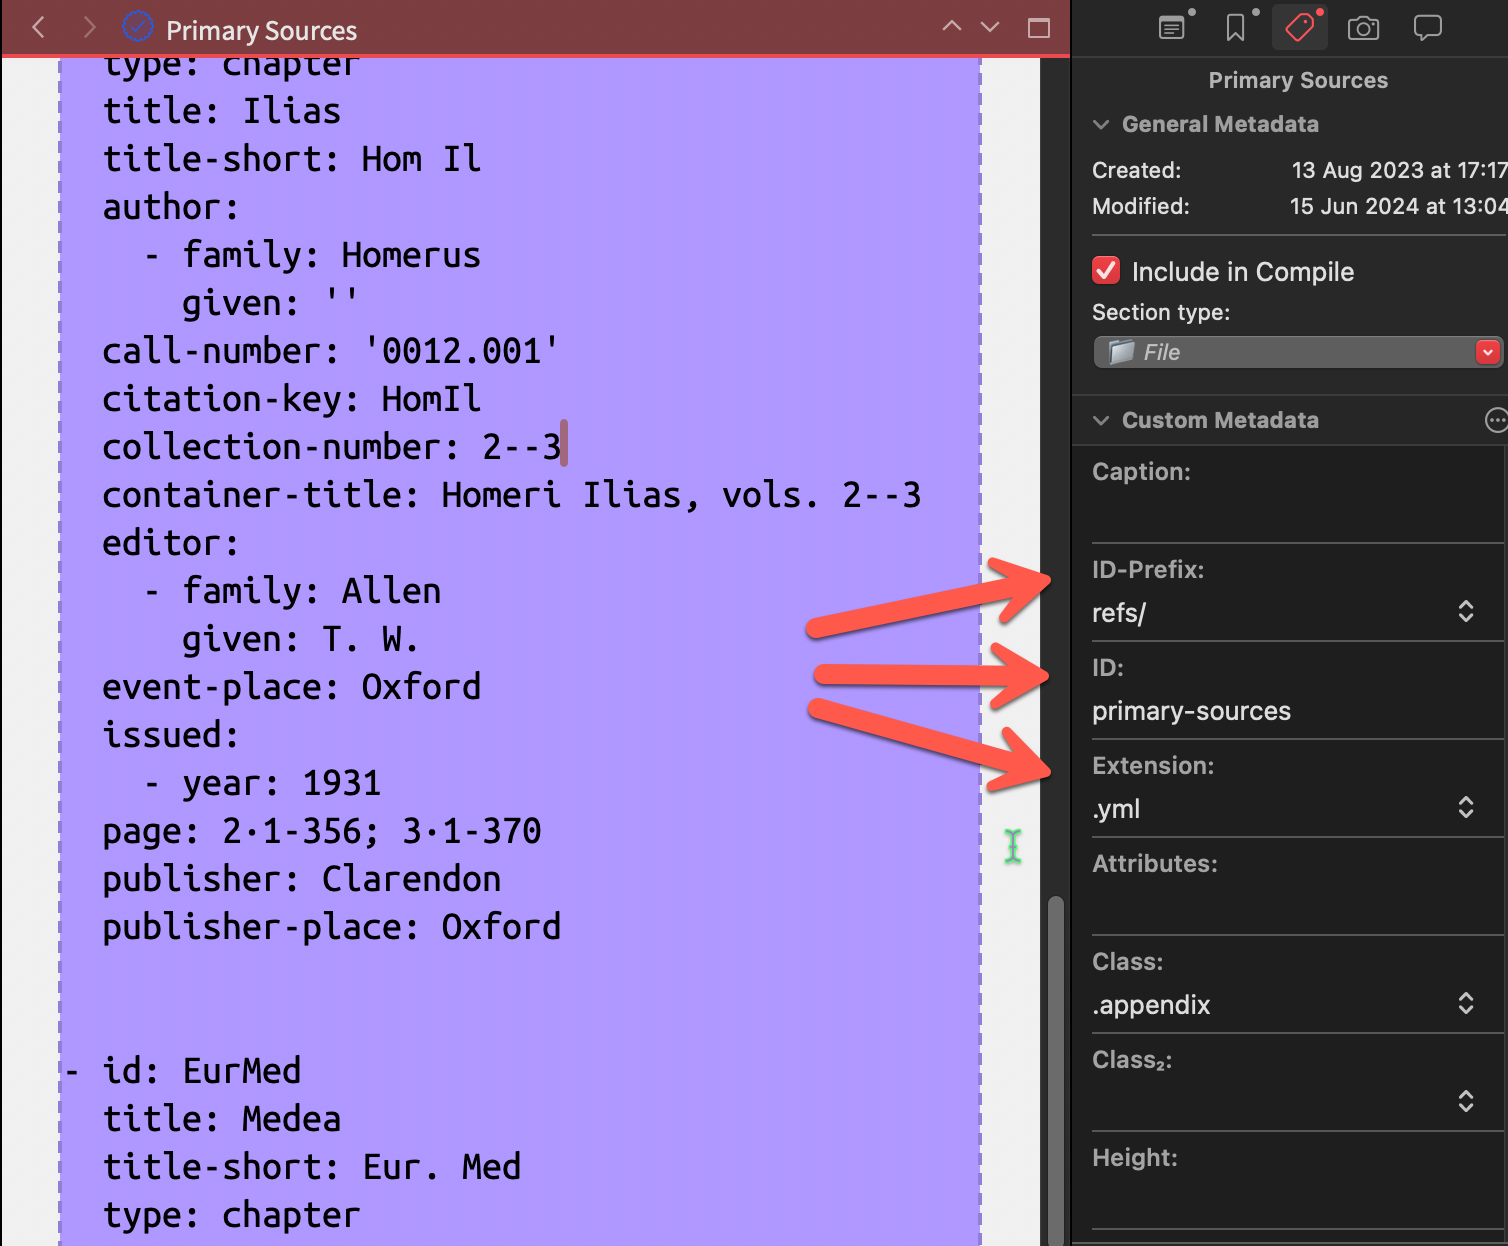
\includegraphics[keepaspectratio]{BibliographyFile.png}}

}

\caption{\label{fig-bibliography}The Metadata panel}

\end{figure}%

\begin{enumerate}
\def\labelenumi{\arabic{enumi}.}
\setcounter{enumi}{2}
\tightlist
\item
  We need to tell Quarto about the bibliography file by adding it to the
  \href{_quarto.yml}{\_quarto} configuration file (there is a
  bibliography section), then we can print the formatted bibliography
  using the ID (\emph{e.g.} \enquote{primary-sources}) with the
  \textbf{Paragraph Style} \emph{Div Bibliography}.
\end{enumerate}

\phantomsection\label{refs_primary-sources}
\begin{CSLReferences}{0}{1}
\bibitem[\citeproctext]{ref-DA}
ARISTOTELIS. {``De Anima''}. Em: BEKKER, I. (Ed.). \emph{Aristotelis
Opera}. Trad.: Β. Τατάκης. Berlin: Reimer, 1834.
{[}\Acrobatmenu{GoBack}{$\hookleftarrow$},
\hyperref[cite_13]{\pageref{cite_13}},
\hyperref[cite_14]{\pageref{cite_14}},
\hyperref[cite_15]{\pageref{cite_15}},
\hyperref[cite_16]{\pageref{cite_16}},
\hyperref[cite_17]{\pageref{cite_17}},
\hyperref[cite_18]{\pageref{cite_18}},
\hyperref[cite_19]{\pageref{cite_19}},
\hyperref[cite_20]{\pageref{cite_20}},
\hyperref[cite_21]{\pageref{cite_21}},
\hyperref[cite_22]{\pageref{cite_22}},
\hyperref[cite_23]{\pageref{cite_23}},
\hyperref[cite_24]{\pageref{cite_24}},
\hyperref[cite_25]{\pageref{cite_25}}{]}

\end{CSLReferences}

\subsection{How to automatically create a multipart
bibliography}\label{nte-multibib2}

We can use the \textbf{Section Type} Bibliography to automate steps 3
and 4. This is very convenient for books that need the bibliography to
print only once at the very end.

\begin{enumerate}
\def\labelenumi{\arabic{enumi}.}
\tightlist
\item
  Using the \textbf{Section Type} File, we create a representation of
  our bibliography file to add the data (\emph{e.g.}
  \href{refs/primary-sources.yml}{Primary Sources} and
  \href{refs/secondary-sources.yml}{Secondary Sources}).
\item
  On the Metadata panel we set the relative path (ID-Prefix + ID) and
  the extension (Extension) of the actual bibliography file that will be
  created upon \textbf{Compile}.
\item
  The metadata with the file path will be automatically added and the
  formatted bibliography will be printed in the same section as the
  data, with the same section title.
\end{enumerate}

\section{Backlinks}\label{backlinks}

In Citeproc, \texttt{link-citations} control whether citations in the
body of the text should be clickable links to the reference in the
bibliography. \textbf{Cite Tools} takes it further and adds a backlink
to each citation an entry has received in the document in a crescent
ordinal fashion\footnote{The reader will see the page number instead of
  a crescent ordinal number in some output formats, such as PDF.}. This
allows the reader to easily arrive at sections of the text where the
same reference was discussed and quickly see how many times each
reference was used with the array of backlinks.

\begin{figure}

\centering{

\pandocbounded{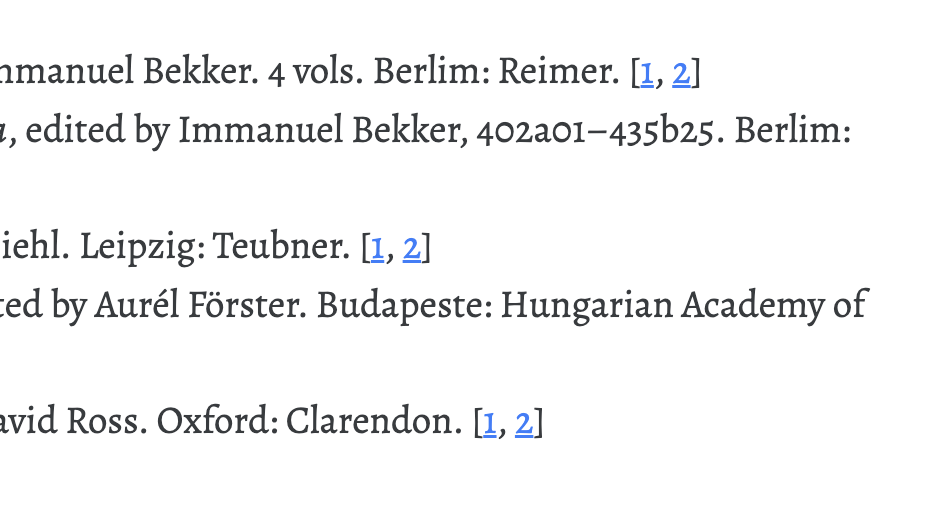
\includegraphics[keepaspectratio]{backrefs.png}}

}

\caption{\label{fig-scrivlinkC}The \textbf{Citation Backlinks} filter
adds an index of cited references to the bibliography, with links back
to all in-text citations. It also allows the user to turn these off
globally or in an \emph{ad hoc} fashion.}

\end{figure}%

\begin{tcolorbox}[enhanced jigsaw, bottomrule=.15mm, bottomtitle=1mm, rightrule=.15mm, opacityback=0, coltitle=black, colback=white, left=2mm, arc=.35mm, colbacktitle=quarto-callout-tip-color!10!white, breakable, toptitle=1mm, colframe=quarto-callout-tip-color-frame, toprule=.15mm, titlerule=0mm, title=\textcolor{quarto-callout-tip-color}{\faLightbulb}\hspace{0.5em}{Turning off undesired linking}, leftrule=.75mm, opacitybacktitle=0.6]

If you want to avoid undesired linking when citing specific fields, turn
\texttt{link-fields} into false

\end{tcolorbox}

\begin{tcolorbox}[enhanced jigsaw, bottomrule=.15mm, bottomtitle=1mm, rightrule=.15mm, opacityback=0, coltitle=black, colback=white, left=2mm, arc=.35mm, colbacktitle=quarto-callout-note-color!10!white, breakable, toptitle=1mm, colframe=quarto-callout-note-color-frame, toprule=.15mm, titlerule=0mm, title=\textcolor{quarto-callout-note-color}{\faInfo}\hspace{0.5em}{Bibliography links}, leftrule=.75mm, opacitybacktitle=0.6]

\ul{link-citations}: Hyperlink citations to the corresponding
bibliography entries. Defaults to true.

\ul{link-fields}: Hyperlink citations targeting specific CSL fields to
the corresponding entries in the bibliography. Defaults to true.

\ul{link-bibliography}: Hyperlink DOIs, PMCIDs, PMID, and URLs in
bibliographies. Defaults to true.

\ul{lang}: Affects the bibliography tags. Defaults to \texttt{en-US}.

\end{tcolorbox}

\chapter{Quarto}\label{quarto}

\section{Scrivener Project Templates}\label{scrivener-project-templates}

All sorts of internal \textbf{Scrivener Templates} have been included
for convenience. They serve as starting points to create new sections.
Click \textbf{Project \textgreater{} New From Template} and select the
desired \textbf{Section Types} from the list, which includes
Bibliography, Code, Computation, Diagram Dot, Diagram Mermaid, Div,
Equation, File, Metadata, Section, Text, Text (Anchored)\footnote{Text
  section with ID for cross-referencing.}.

This provides a huge number of options as the metadata can be customized
to create many \textbf{Quarto} elements. Using the \textbf{Section Type}
\textbf{Div}, for example, one could create 8 different \textbf{Amsthm}
elements, 5 different \textbf{Callouts}, and several \textbf{Column}
environments. Using the \textbf{Computation}, one can create executable
code blocks with R, Python, and Ruby. The \textbf{Section} \textbf{Type}
\textbf{Section} can be numbered, unnumbered, or part of the appendix
(with the use of classes).

Look at the ready-made examples to see what else is possible.

\section{Cross-referencing}\label{cross-referencing}

When a \textbf{Section} is created, select the correct
\texttt{ID-Prefix} (\emph{e.g.} \texttt{sec-}), and fill the \texttt{ID}
metadata field with a value (\emph{e.g.} \texttt{xref}). Then, use
Scrivener placeholders, such as
\texttt{@\textless{}\textbackslash{}\$Custom:ID-Prefix\textgreater{}\textless{}\textbackslash{}\$Custom:ID\textgreater{}}
with a link to the cited element, so that this gets replaced with
\texttt{\textbackslash{}@sec-xref}. This works regardless of the element
being cross-referenced (\emph{e.g.} \emph{section}, \emph{table},
\emph{figure}, \emph{listing}) because this strategy ensures the
citation will use the
\texttt{\textless{}\textbackslash{}\$Custom:ID-Prefix\textgreater{}}
pulled from the targeted element (\emph{e.g.} \texttt{sec-},
\texttt{tbl-}, \texttt{fig-}, \texttt{lst-}), making it compatible with
all element types.

\begin{tcolorbox}[enhanced jigsaw, bottomrule=.15mm, bottomtitle=1mm, rightrule=.15mm, opacityback=0, coltitle=black, colback=white, left=2mm, arc=.35mm, colbacktitle=quarto-callout-warning-color!10!white, breakable, toptitle=1mm, colframe=quarto-callout-warning-color-frame, toprule=.15mm, titlerule=0mm, title=\textcolor{quarto-callout-warning-color}{\faExclamationTriangle}\hspace{0.5em}{Link anchor}, leftrule=.75mm, opacitybacktitle=0.6]

To be less verbose, we have set up a replacement rule that allows a
shorter label to be used as the link anchor.

\begin{itemize}
\tightlist
\item
  \texttt{s\textbackslash{}crivlink} is replaced with
  \texttt{\textless{}\textbackslash{}\$Custom:ID-Prefix\textgreater{}\textless{}\textbackslash{}\$Custom:ID\textgreater{}}.
\item
  \texttt{s\textbackslash{}crivpath} and \texttt{\$\textbackslash{}!}
  are replaced with
  \texttt{\textless{}\textbackslash{}\$Custom:ID-Prefix\textgreater{}\textless{}\textbackslash{}\$Custom:ID\textgreater{}\textless{}\textbackslash{}\$Custom:Extension\textgreater{}}.
\end{itemize}

\end{tcolorbox}

\begin{tcolorbox}[enhanced jigsaw, bottomrule=.15mm, bottomtitle=1mm, rightrule=.15mm, opacityback=0, coltitle=black, colback=white, left=2mm, arc=.35mm, colbacktitle=quarto-callout-tip-color!10!white, breakable, toptitle=1mm, colframe=quarto-callout-tip-color-frame, toprule=.15mm, titlerule=0mm, title=\textcolor{quarto-callout-tip-color}{\faLightbulb}\hspace{0.5em}{Cross-referencing an element}, leftrule=.75mm, opacitybacktitle=0.6]

\begin{enumerate}
\def\labelenumi{\arabic{enumi}.}
\tightlist
\item
  Type \ul{your-keyword-of-choice} or
  \texttt{s\textbackslash{}crivlink}, select it, and hit \ul{Command +
  L};
\item
  Link to the document that contains the table.
\item
  Apply a \textbf{Character Style} called \emph{Cite}.
\end{enumerate}

\end{tcolorbox}

\begin{tcolorbox}[enhanced jigsaw, bottomrule=.15mm, bottomtitle=1mm, rightrule=.15mm, opacityback=0, coltitle=black, colback=white, left=2mm, arc=.35mm, colbacktitle=quarto-callout-caution-color!10!white, breakable, toptitle=1mm, colframe=quarto-callout-caution-color-frame, toprule=.15mm, titlerule=0mm, title=\textcolor{quarto-callout-caution-color}{\faFire}\hspace{0.5em}{Known limitation}, leftrule=.75mm, opacitybacktitle=0.6]

\textbf{Scrivener Placeholders} can only pull information from the
section properties, so this works when we are referencing elements
created using \textbf{Section Types}.

When referencing elements created using \textbf{Raw Markup} or a
\textbf{Character Style}, we must use the same \texttt{ID} we gave the
element (\emph{e.g.} \texttt{fig-ulysses}) instead of our generic link
label (\emph{e.g.} \texttt{s\textbackslash{}crivlink}).

\end{tcolorbox}

\section{Amsthm}\label{amsthm}

\begin{longtable}[]{@{}ccc@{}}
\toprule\noalign{}
\textbf{Species} & \textbf{Markdown Source} & \textbf{Rendered
Output} \\
\midrule\noalign{}
\endfirsthead
\toprule\noalign{}
\textbf{Species} & \textbf{Markdown Source} & \textbf{Rendered
Output} \\
\midrule\noalign{}
\endhead
\bottomrule\noalign{}
\tabularnewline
\caption{Cross-referencing \textbf{Amsthm} elements in
ScrivQ.}\label{tbl-amsthm}\tabularnewline
\endlastfoot
Conjecture & \texttt{{[}@cnj-demo{]}} &
\phantomsection\label{cite_30}{\label{cite_30}Conjecture~\ref{cnj-demo}} \\
Corollary & \texttt{{[}@cor-demo{]}} &
\phantomsection\label{cite_31}{\label{cite_31}Corollary~\ref{cor-demo}} \\
Definition & \texttt{{[}@def-demo{]}} &
\phantomsection\label{cite_32}{\label{cite_32}Definition~\ref{def-demo}} \\
Example & \texttt{{[}@exm-demo{]}} &
\phantomsection\label{cite_33}{\label{cite_33}Example~\ref{exm-demo}} \\
Exercise & \texttt{{[}@exr-demo{]}} &
\phantomsection\label{cite_34}{\label{cite_34}Exercise~\ref{exr-demo}} \\
Lemma & \texttt{{[}@lem-demo{]}} &
\phantomsection\label{cite_35}{\label{cite_35}Lemma~\ref{lem-demo}} \\
Proposition & \texttt{{[}@prp-demo{]}} &
\phantomsection\label{cite_36}{\label{cite_36}Proposition~\ref{prp-demo}} \\
Theorem & \texttt{{[}@thm-demo{]}} &
\phantomsection\label{cite_37}{\label{cite_37}Theorem~\ref{thm-demo}} \\
\end{longtable}

\begin{conjecture}[]\protect\hypertarget{cnj-demo}{}\label{cnj-demo}

Demonstration of the \textbf{Conjecture} theorem environment using the
\textbf{Section Type} \texttt{Div} with \textbf{ID} \texttt{\#cnj-demo}.

\end{conjecture}

\begin{corollary}[]\protect\hypertarget{cor-demo}{}\label{cor-demo}

Demonstration of the \textbf{Corollary} theorem environment using the
\textbf{Section Type} \texttt{Div} with \textbf{ID} \texttt{\#cor-demo}.

\end{corollary}

\begin{definition}[]\protect\hypertarget{def-demo}{}\label{def-demo}

Demonstration of the \textbf{Definition} theorem environment using the
\textbf{Section Type} \texttt{Div} with \textbf{ID} \texttt{\#def-demo}.

\end{definition}

\begin{example}[]\protect\hypertarget{exm-demo}{}\label{exm-demo}

Demonstration of the \textbf{Example} theorem environment using the
\textbf{Section Type} \texttt{Div} with \textbf{ID} \texttt{\#exm-demo}.

\end{example}

\begin{exercise}[]\protect\hypertarget{exr-demo}{}\label{exr-demo}

Demonstration of the \textbf{Exercise} theorem environment using the
\textbf{Section Type} \texttt{Div} with \textbf{ID} \texttt{\#exr-demo}.

\end{exercise}

\begin{lemma}[]\protect\hypertarget{lem-demo}{}\label{lem-demo}

Demonstration of the \textbf{Lemma} theorem environment using the
\textbf{Section Type} \texttt{Div} with \textbf{ID} \texttt{\#lem-demo}.

\end{lemma}

\begin{proposition}[]\protect\hypertarget{prp-demo}{}\label{prp-demo}

Demonstration of the \textbf{Proposition} theorem environment using the
\textbf{Section Type} \texttt{Div} with \textbf{ID} \texttt{\#prp-demo}.

\end{proposition}

\begin{theorem}[]\protect\hypertarget{thm-demo}{}\label{thm-demo}

Demonstration of the \textbf{Theorem} theorem environment using the
\textbf{Section Type} \texttt{Div} with \textbf{ID} \texttt{\#thm-demo}.

\[[ x^2 + y^2 = z^2 ]\]

\end{theorem}

\section{Callouts}\label{callouts}

\begin{longtable}[]{@{}ccc@{}}
\toprule\noalign{}
\textbf{Species} & \textbf{Markdown Source} & \textbf{Rendered
Output} \\
\midrule\noalign{}
\endfirsthead
\toprule\noalign{}
\textbf{Species} & \textbf{Markdown Source} & \textbf{Rendered
Output} \\
\midrule\noalign{}
\endhead
\bottomrule\noalign{}
\tabularnewline
\caption{Cross-referencing callouts.}\label{tbl-callouts}\tabularnewline
\endlastfoot
Caution & \texttt{{[}@cau-caution{]}} &
\phantomsection\label{cite_38}{\label{cite_38}Caution~\ref{cau-caution}} \\
Important & \texttt{{[}@imp-important{]}} &
\phantomsection\label{cite_39}{\label{cite_39}Important~\ref{imp-important}} \\
Note & \texttt{{[}@nte-note{]}} &
\phantomsection\label{cite_40}{\label{cite_40}Note~\ref{nte-note}} \\
Tip & \texttt{{[}@tip-tip{]}} &
\phantomsection\label{cite_41}{\label{cite_41}Tip~\ref{tip-tip}} \\
Warning & \texttt{{[}@wrn-warning{]}} &
\phantomsection\label{cite_42}{\label{cite_42}Warning~\ref{wrn-warning}} \\
\end{longtable}

Using styles, you can create normal or collapsed callouts.

\begin{tcolorbox}[enhanced jigsaw, bottomrule=.15mm, bottomtitle=1mm, rightrule=.15mm, opacityback=0, coltitle=black, colback=white, left=2mm, arc=.35mm, colbacktitle=quarto-callout-caution-color!10!white, breakable, toptitle=1mm, colframe=quarto-callout-caution-color-frame, toprule=.15mm, titlerule=0mm, title=\textcolor{quarto-callout-caution-color}{\faFire}\hspace{0.5em}{Caution (collapsed)}, leftrule=.75mm, opacitybacktitle=0.6]

This is a Callout Caution using a \textbf{Paragraph Style}.

\end{tcolorbox}

\begin{tcolorbox}[enhanced jigsaw, bottomrule=.15mm, bottomtitle=1mm, rightrule=.15mm, opacityback=0, coltitle=black, colback=white, left=2mm, arc=.35mm, colbacktitle=quarto-callout-caution-color!10!white, breakable, toptitle=1mm, colframe=quarto-callout-caution-color-frame, toprule=.15mm, titlerule=0mm, title=\textcolor{quarto-callout-caution-color}{\faFire}\hspace{0.5em}{Caution}, leftrule=.75mm, opacitybacktitle=0.6]

This is a Callout Caution using a \textbf{Paragraph Style}.

\end{tcolorbox}

\begin{tcolorbox}[enhanced jigsaw, bottomrule=.15mm, arc=.35mm, rightrule=.15mm, breakable, colframe=quarto-callout-caution-color-frame, toprule=.15mm, colback=white, left=2mm, leftrule=.75mm, opacityback=0]
\begin{minipage}[t]{5.5mm}
\textcolor{quarto-callout-caution-color}{\faFire}
\end{minipage}%
\begin{minipage}[t]{\textwidth - 5.5mm}

\quartocalloutcau{cau-caution} 

\vspace{-3mm}\textbf{Caution \ref*{cau-caution} }\vspace{3mm}

Demonstration of a \textbf{Callout Caution} using the \textbf{Section
Type} \texttt{Div} with class \texttt{.callout-caution} and with
\textbf{ID} \texttt{\#cau-caution}.

\end{minipage}%
\end{tcolorbox}

\begin{tcolorbox}[enhanced jigsaw, bottomrule=.15mm, arc=.35mm, rightrule=.15mm, breakable, colframe=quarto-callout-important-color-frame, toprule=.15mm, colback=white, left=2mm, leftrule=.75mm, opacityback=0]
\begin{minipage}[t]{5.5mm}
\textcolor{quarto-callout-important-color}{\faExclamation}
\end{minipage}%
\begin{minipage}[t]{\textwidth - 5.5mm}

\quartocalloutimp{imp-important} 

\vspace{-3mm}\textbf{Important \ref*{imp-important} }\vspace{3mm}

Demonstration of a \textbf{Callout Important} using the \textbf{Section
Type} \texttt{Div} with class \texttt{.callout-important} and with
\textbf{ID} \texttt{\#imp-important}.

\end{minipage}%
\end{tcolorbox}

\begin{tcolorbox}[enhanced jigsaw, bottomrule=.15mm, arc=.35mm, rightrule=.15mm, breakable, colframe=quarto-callout-note-color-frame, toprule=.15mm, colback=white, left=2mm, leftrule=.75mm, opacityback=0]
\begin{minipage}[t]{5.5mm}
\textcolor{quarto-callout-note-color}{\faInfo}
\end{minipage}%
\begin{minipage}[t]{\textwidth - 5.5mm}

\quartocalloutnte{nte-note} 

\vspace{-3mm}\textbf{Note \ref*{nte-note} }\vspace{3mm}

Demonstration of a \textbf{Callout Note} using the \textbf{Section Type}
\texttt{Div} with class \texttt{.callout-note} and with \textbf{ID}
\texttt{\#nte-note}.

\end{minipage}%
\end{tcolorbox}

\begin{tcolorbox}[enhanced jigsaw, bottomrule=.15mm, arc=.35mm, rightrule=.15mm, breakable, colframe=quarto-callout-tip-color-frame, toprule=.15mm, colback=white, left=2mm, leftrule=.75mm, opacityback=0]
\begin{minipage}[t]{5.5mm}
\textcolor{quarto-callout-tip-color}{\faLightbulb}
\end{minipage}%
\begin{minipage}[t]{\textwidth - 5.5mm}

\quartocallouttip{tip-tip} 

\vspace{-3mm}\textbf{Tip \ref*{tip-tip} }\vspace{3mm}

Demonstration of a \textbf{Callout Tip} using the \textbf{Section Type}
\texttt{Div} with class \texttt{.callout-tip} and with \textbf{ID}
\texttt{\#tip-tip}.

\end{minipage}%
\end{tcolorbox}

\begin{tcolorbox}[enhanced jigsaw, bottomrule=.15mm, arc=.35mm, rightrule=.15mm, breakable, colframe=quarto-callout-warning-color-frame, toprule=.15mm, colback=white, left=2mm, leftrule=.75mm, opacityback=0]
\begin{minipage}[t]{5.5mm}
\textcolor{quarto-callout-warning-color}{\faExclamationTriangle}
\end{minipage}%
\begin{minipage}[t]{\textwidth - 5.5mm}

\quartocalloutwrn{wrn-warning} 

\vspace{-3mm}\textbf{Warning \ref*{wrn-warning} }\vspace{3mm}

Demonstration of a \textbf{Callout Warning} using the \textbf{Section
Type} \texttt{Div} with class \texttt{.callout-warning} and with
\textbf{ID} \texttt{\#wrn-warning}.

\end{minipage}%
\end{tcolorbox}

\section{Diagrams}\label{diagrams}

Similarly, we can create \textbf{Dot} and \textbf{Mermaid} diagrams
using \textbf{Section Types} (\emph{Diagram Dot}, \emph{Diagram
Mermaid}), \textbf{Paragraph Styles} (\emph{Diagram Dot}, \emph{Diagram
Mermaid}), and \textbf{Raw Mardown}.

\begin{longtable}[]{@{}ccc@{}}
\toprule\noalign{}
\textbf{Species} & \textbf{Markdown Source} & \textbf{Rendered
Output} \\
\midrule\noalign{}
\endfirsthead
\toprule\noalign{}
\textbf{Species} & \textbf{Markdown Source} & \textbf{Rendered
Output} \\
\midrule\noalign{}
\endhead
\bottomrule\noalign{}
\tabularnewline
\caption{Cross-referencing \textbf{Dot} and \textbf{Mermaid}
diagrams.}\label{tbl-diagrams}\tabularnewline
\endlastfoot
Dot & \texttt{{[}@fig-dot-a{]}} &
\phantomsection\label{cite_43}{\label{cite_43}Figure~\ref{fig-dot-a}} \\
Dot & \texttt{{[}@fig-dot-b{]}} &
\phantomsection\label{cite_44}{\label{cite_44}Figure~\ref{fig-dot-b}} \\
Dot & \texttt{{[}@fig-dot-c{]}} &
\phantomsection\label{cite_45}{\label{cite_45}Figure~\ref{fig-dot-c}} \\
Mermaid & \texttt{{[}@fig-mermaid-a{]}} &
\phantomsection\label{cite_46}{\label{cite_46}Figure~\ref{fig-mermaid-a}} \\
Mermaid & \texttt{{[}@fig-mermaid-b{]}} &
\phantomsection\label{cite_47}{\label{cite_47}Figure~\ref{fig-mermaid-b}} \\
Mermaid & \texttt{{[}@fig-mermaid-c{]}} &
\phantomsection\label{cite_48}{\label{cite_48}Figure~\ref{fig-mermaid-c}} \\
\end{longtable}

\begin{figure*}

\centering{

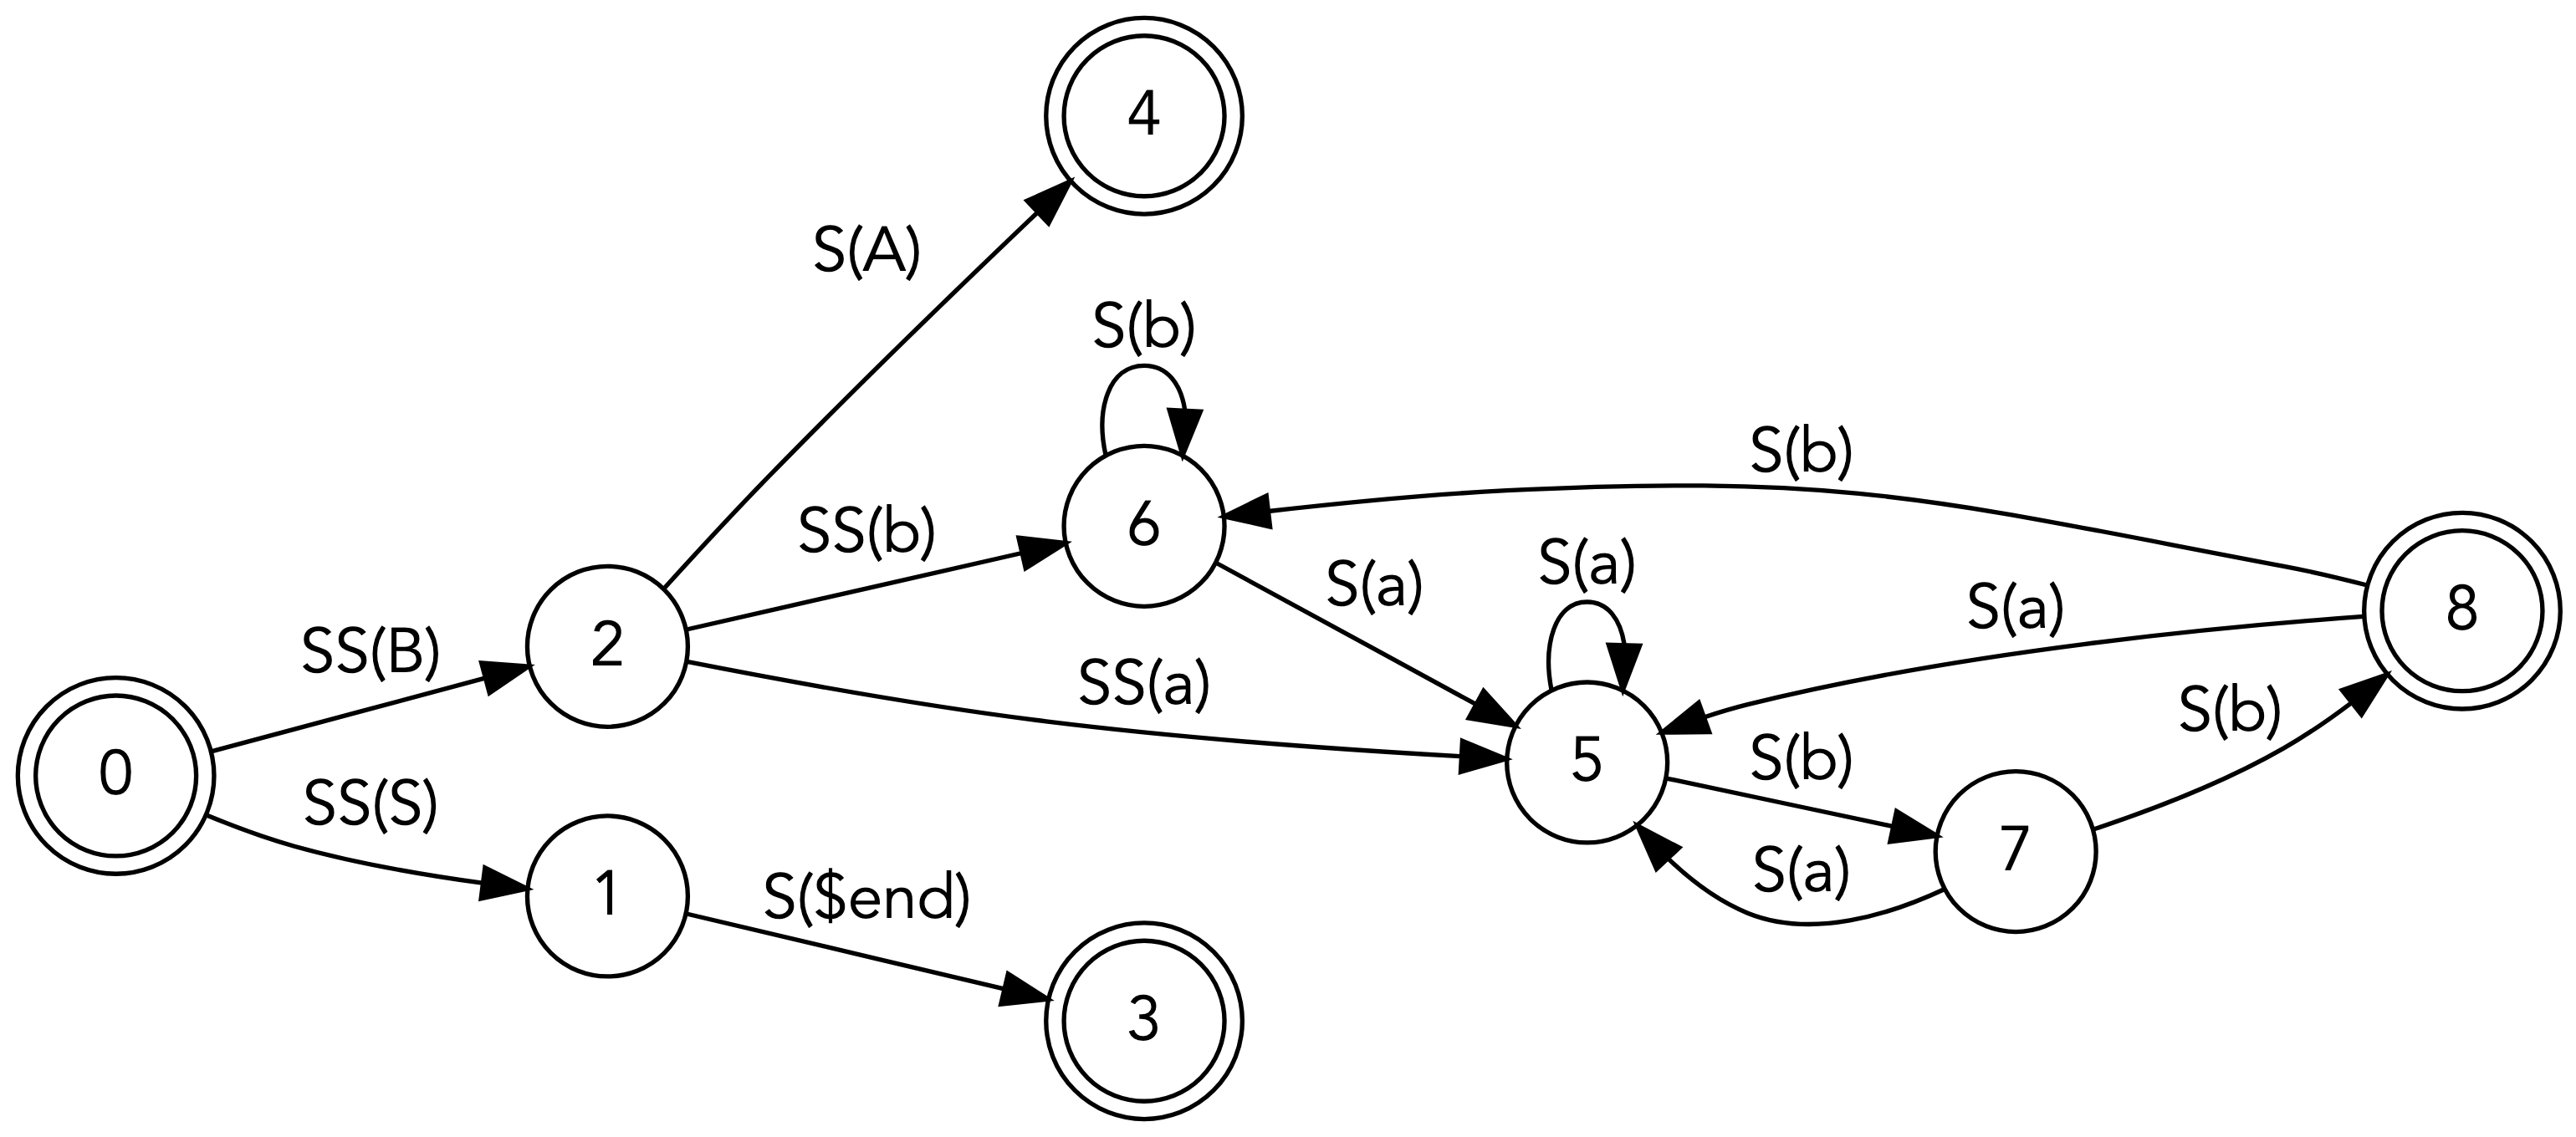
\includegraphics[width=5.5in,height=3.5in]{ScrivQ24_files/figure-latex/dot-figure-1.png}

}

\caption{\label{fig-dot-a}Figure caption}

\end{figure*}%

\begin{figure*}

\centering{

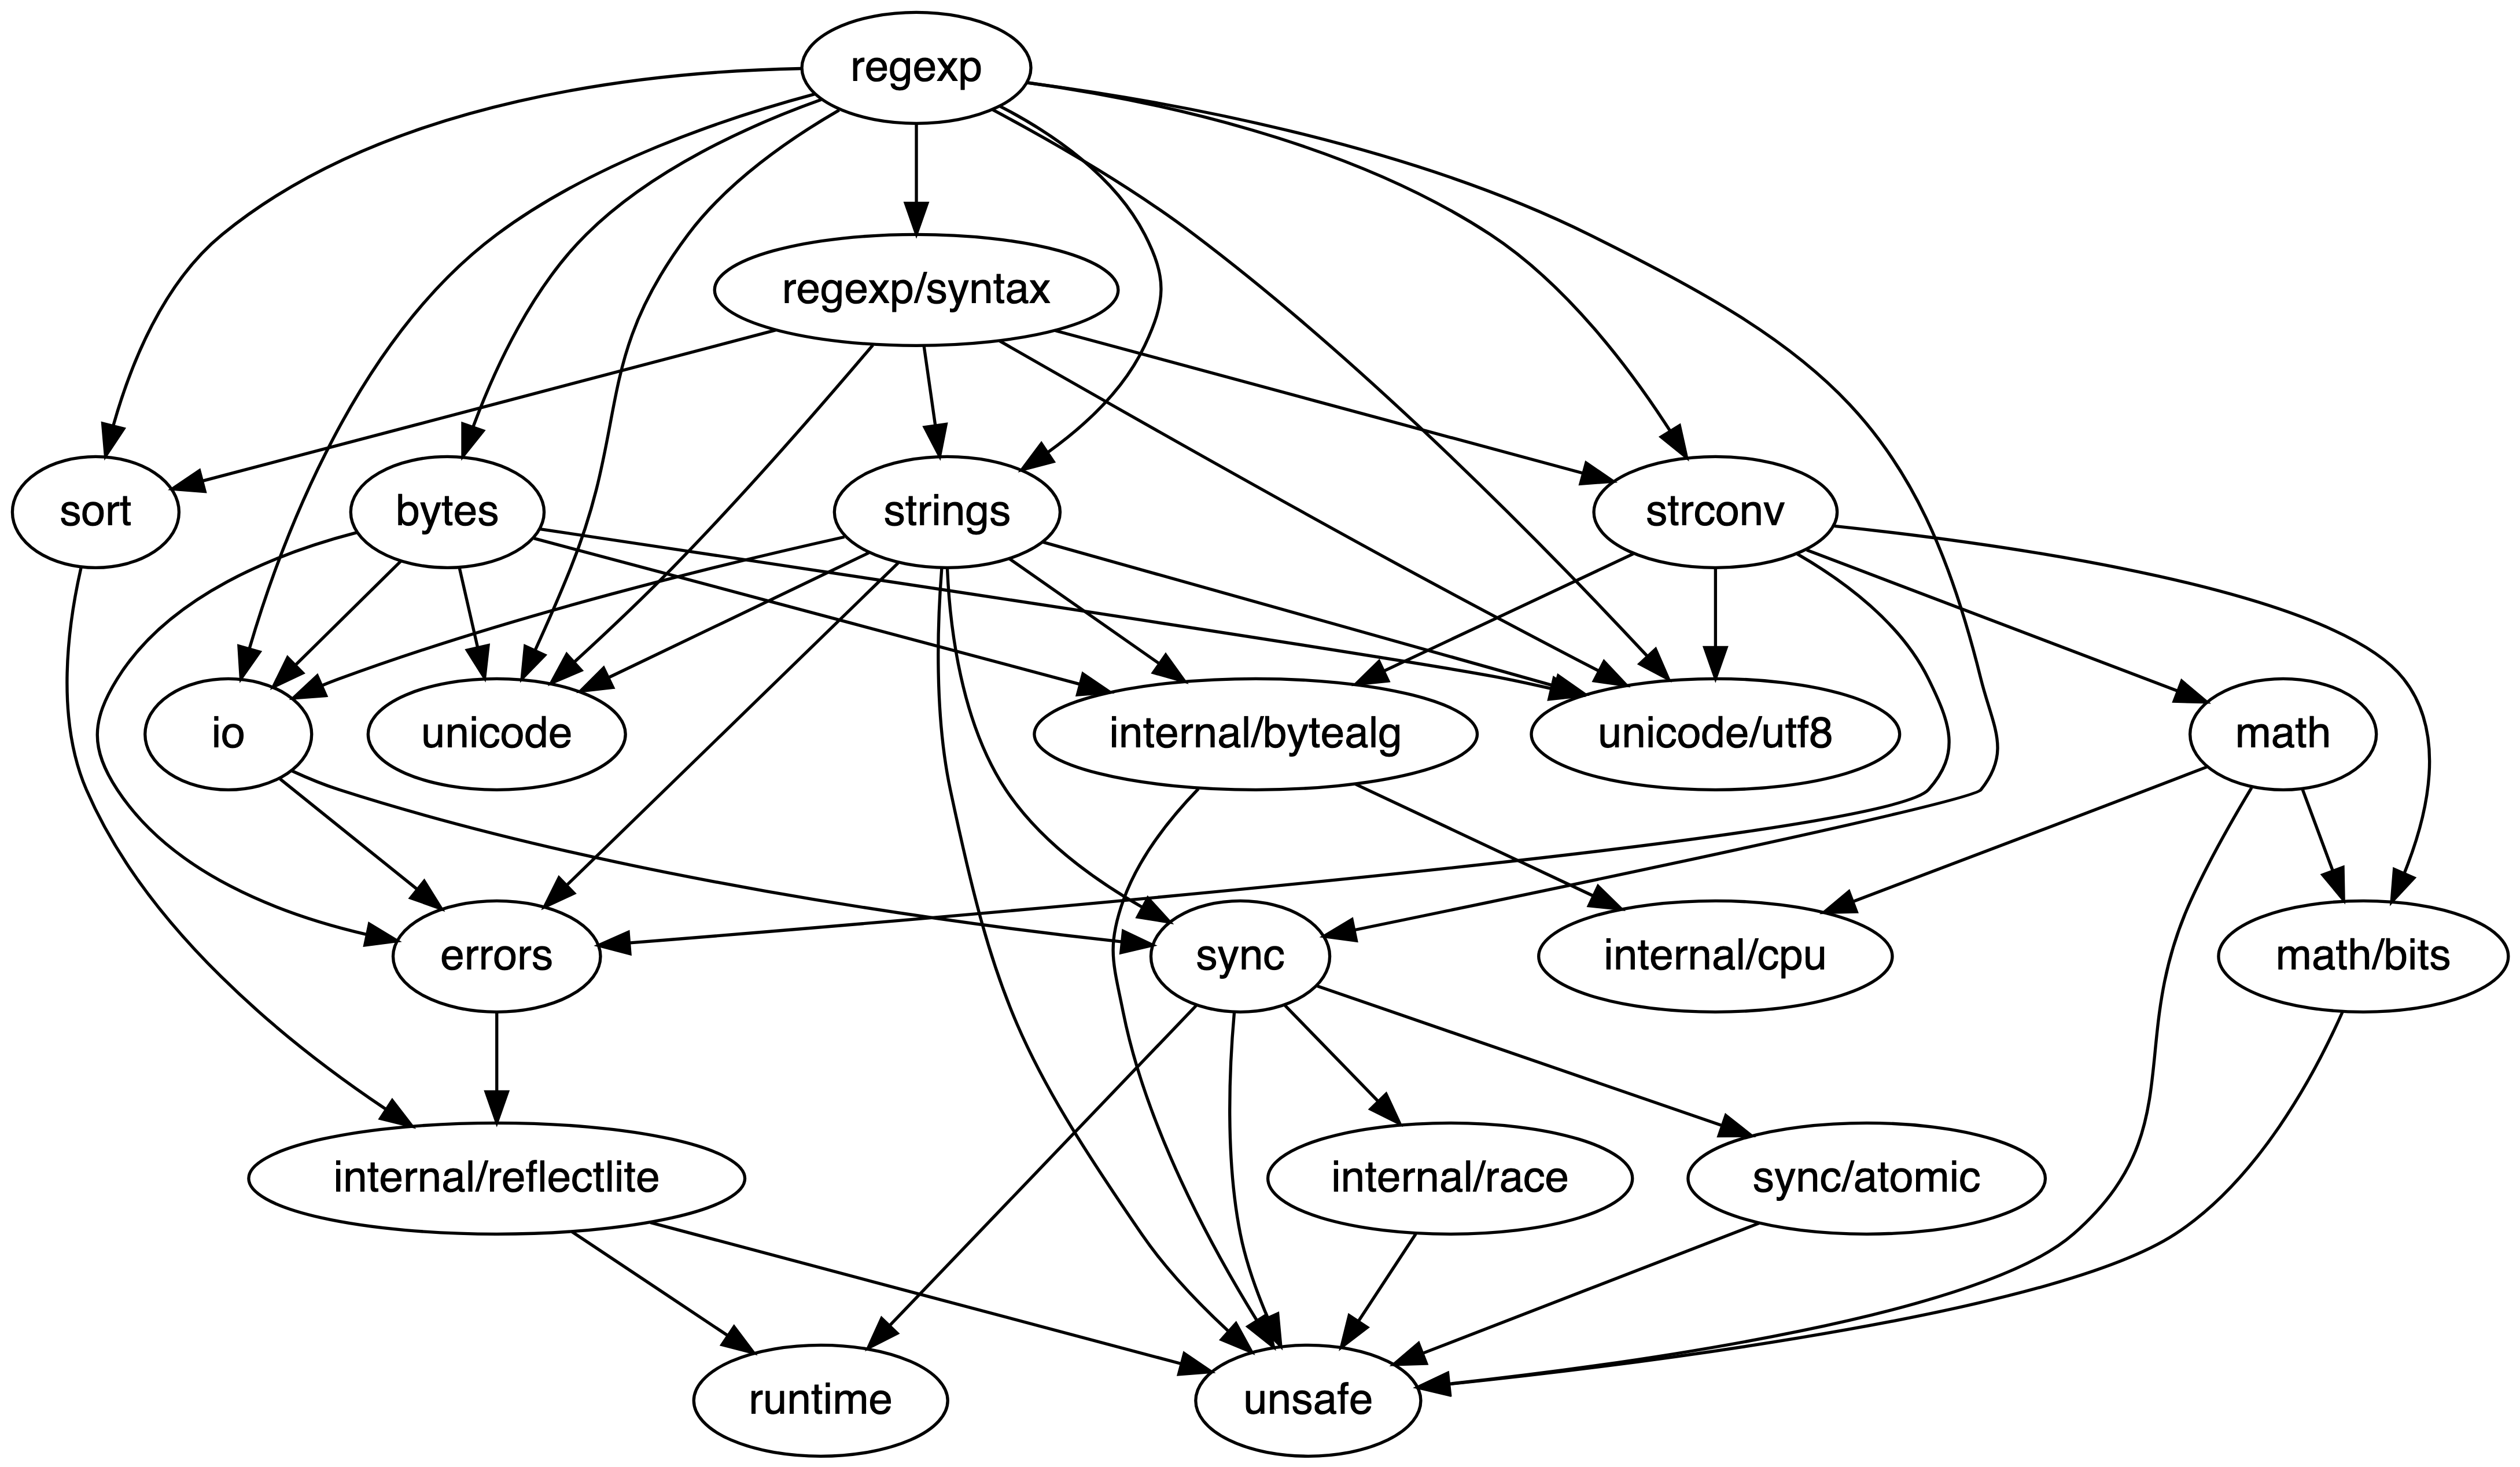
\includegraphics[width=5.5in,height=3.5in]{ScrivQ24_files/figure-latex/dot-figure-3.png}

}

\caption{\label{fig-dot-b}A graphviz graph with figure reference and
caption, using raw markup. See
https://quarto.org/docs/authoring/diagrams.html\#sizing for more
details\ldots{}}

\end{figure*}%

\begin{figure*}

\centering{

\includegraphics[width=5.5in,height=3.5in]{ScrivQ24_files/figure-latex/dot-figure-2.png}

}

\caption{\label{fig-dot-c}Color wheel diagram}

\end{figure*}%

\begin{figure}

\centering{

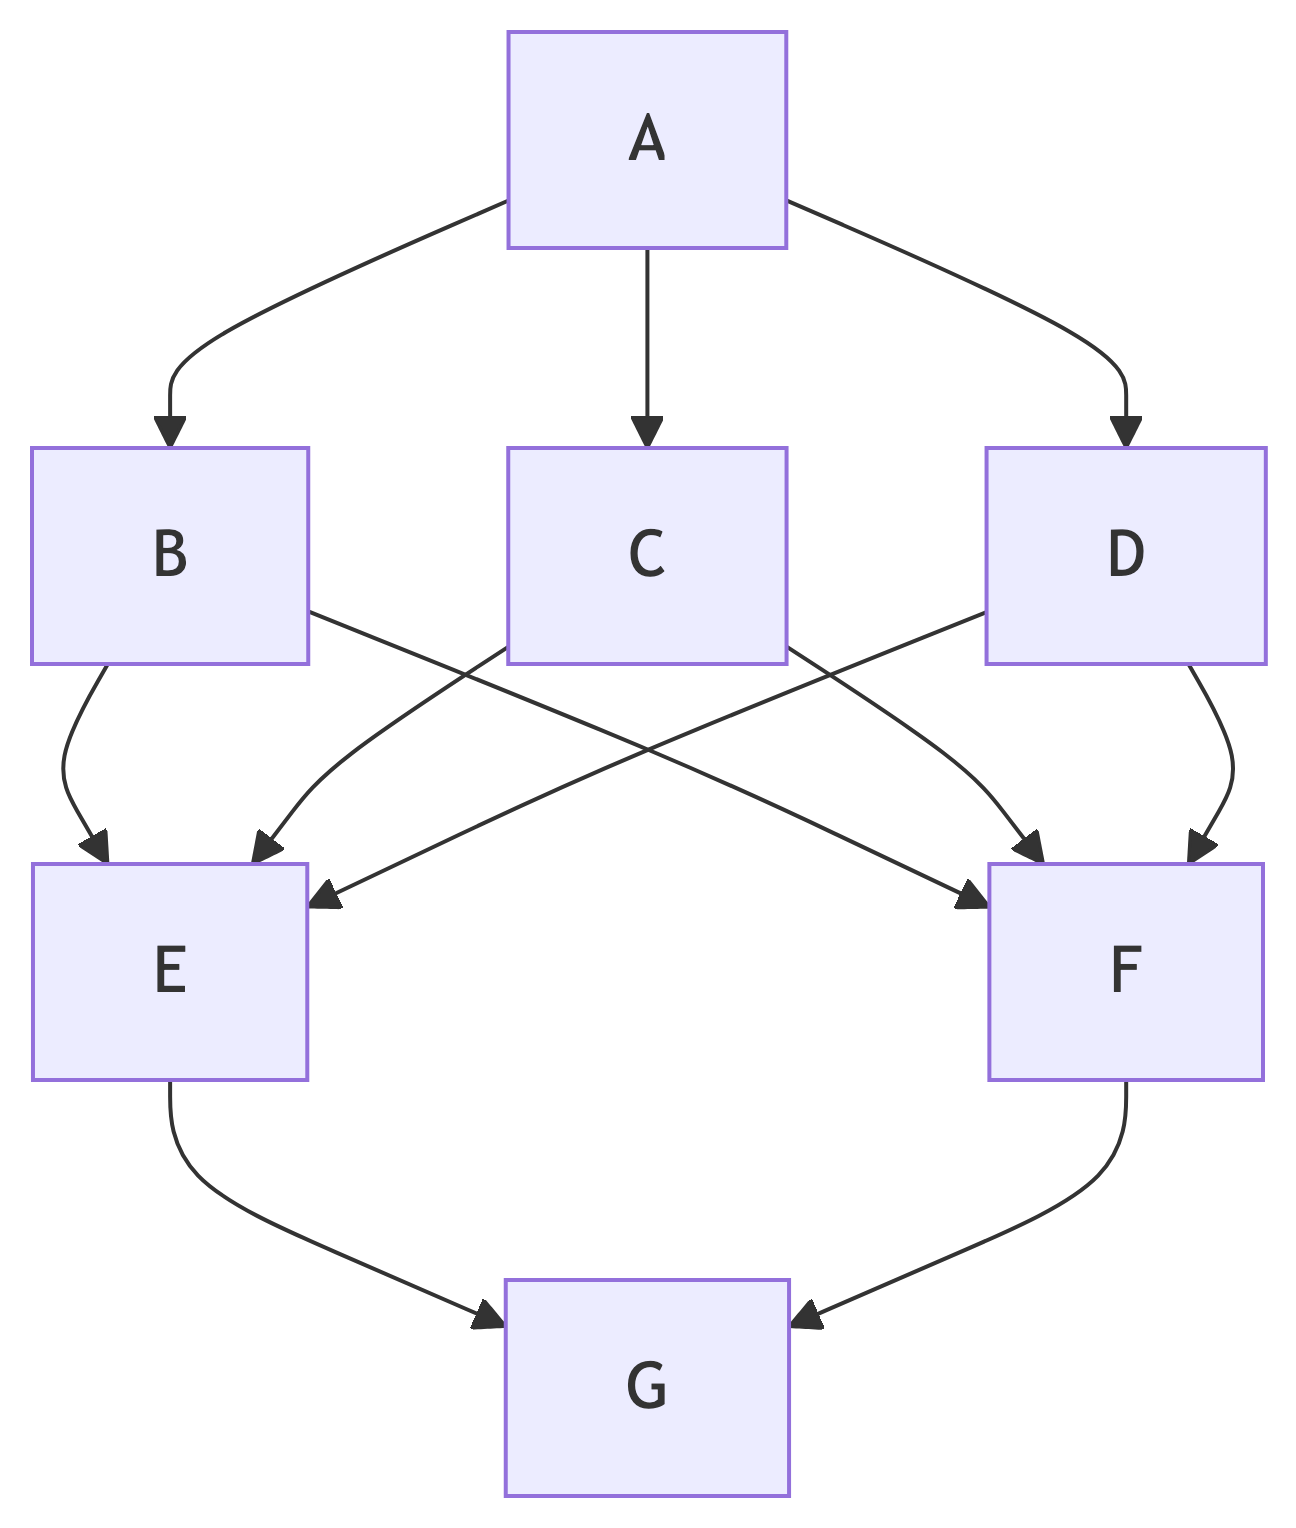
\includegraphics[width=3.38in,height=3.98in]{ScrivQ24_files/figure-latex/mermaid-figure-1.png}

}

\caption{\label{fig-mermaid-a}Figure caption}

\end{figure}%

\begin{figure*}

\centering{

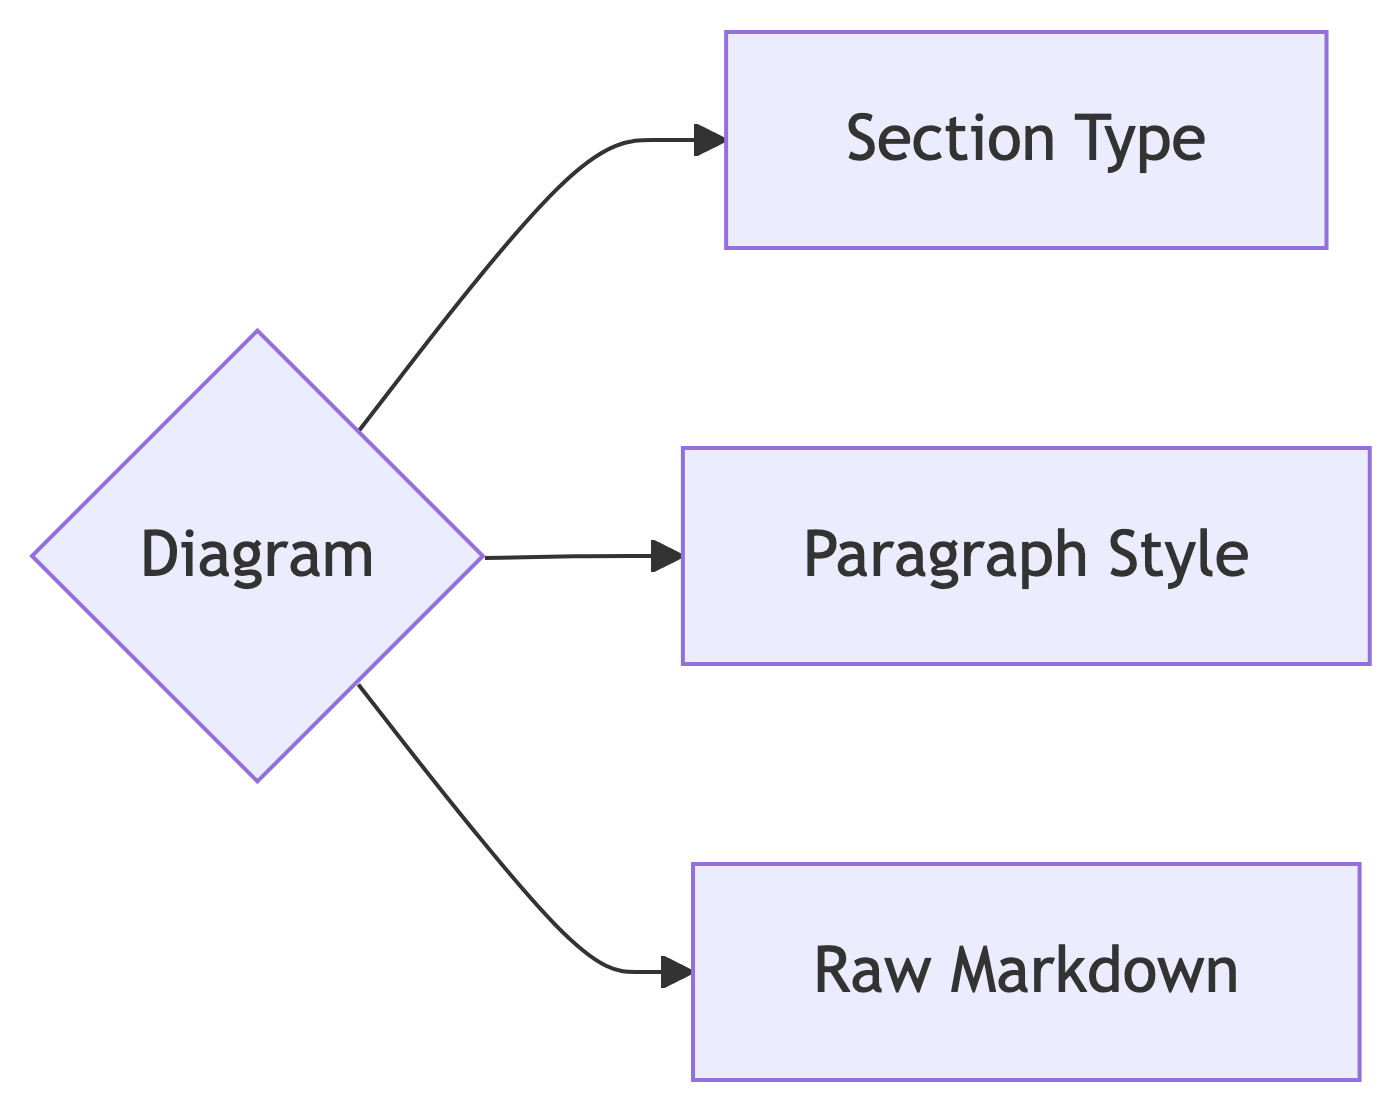
\includegraphics[width=3.65in,height=2.9in]{ScrivQ24_files/figure-latex/mermaid-figure-3.png}

}

\caption{\label{fig-mermaid-b}Figure caption}

\end{figure*}%

\begin{figure}

\centering{

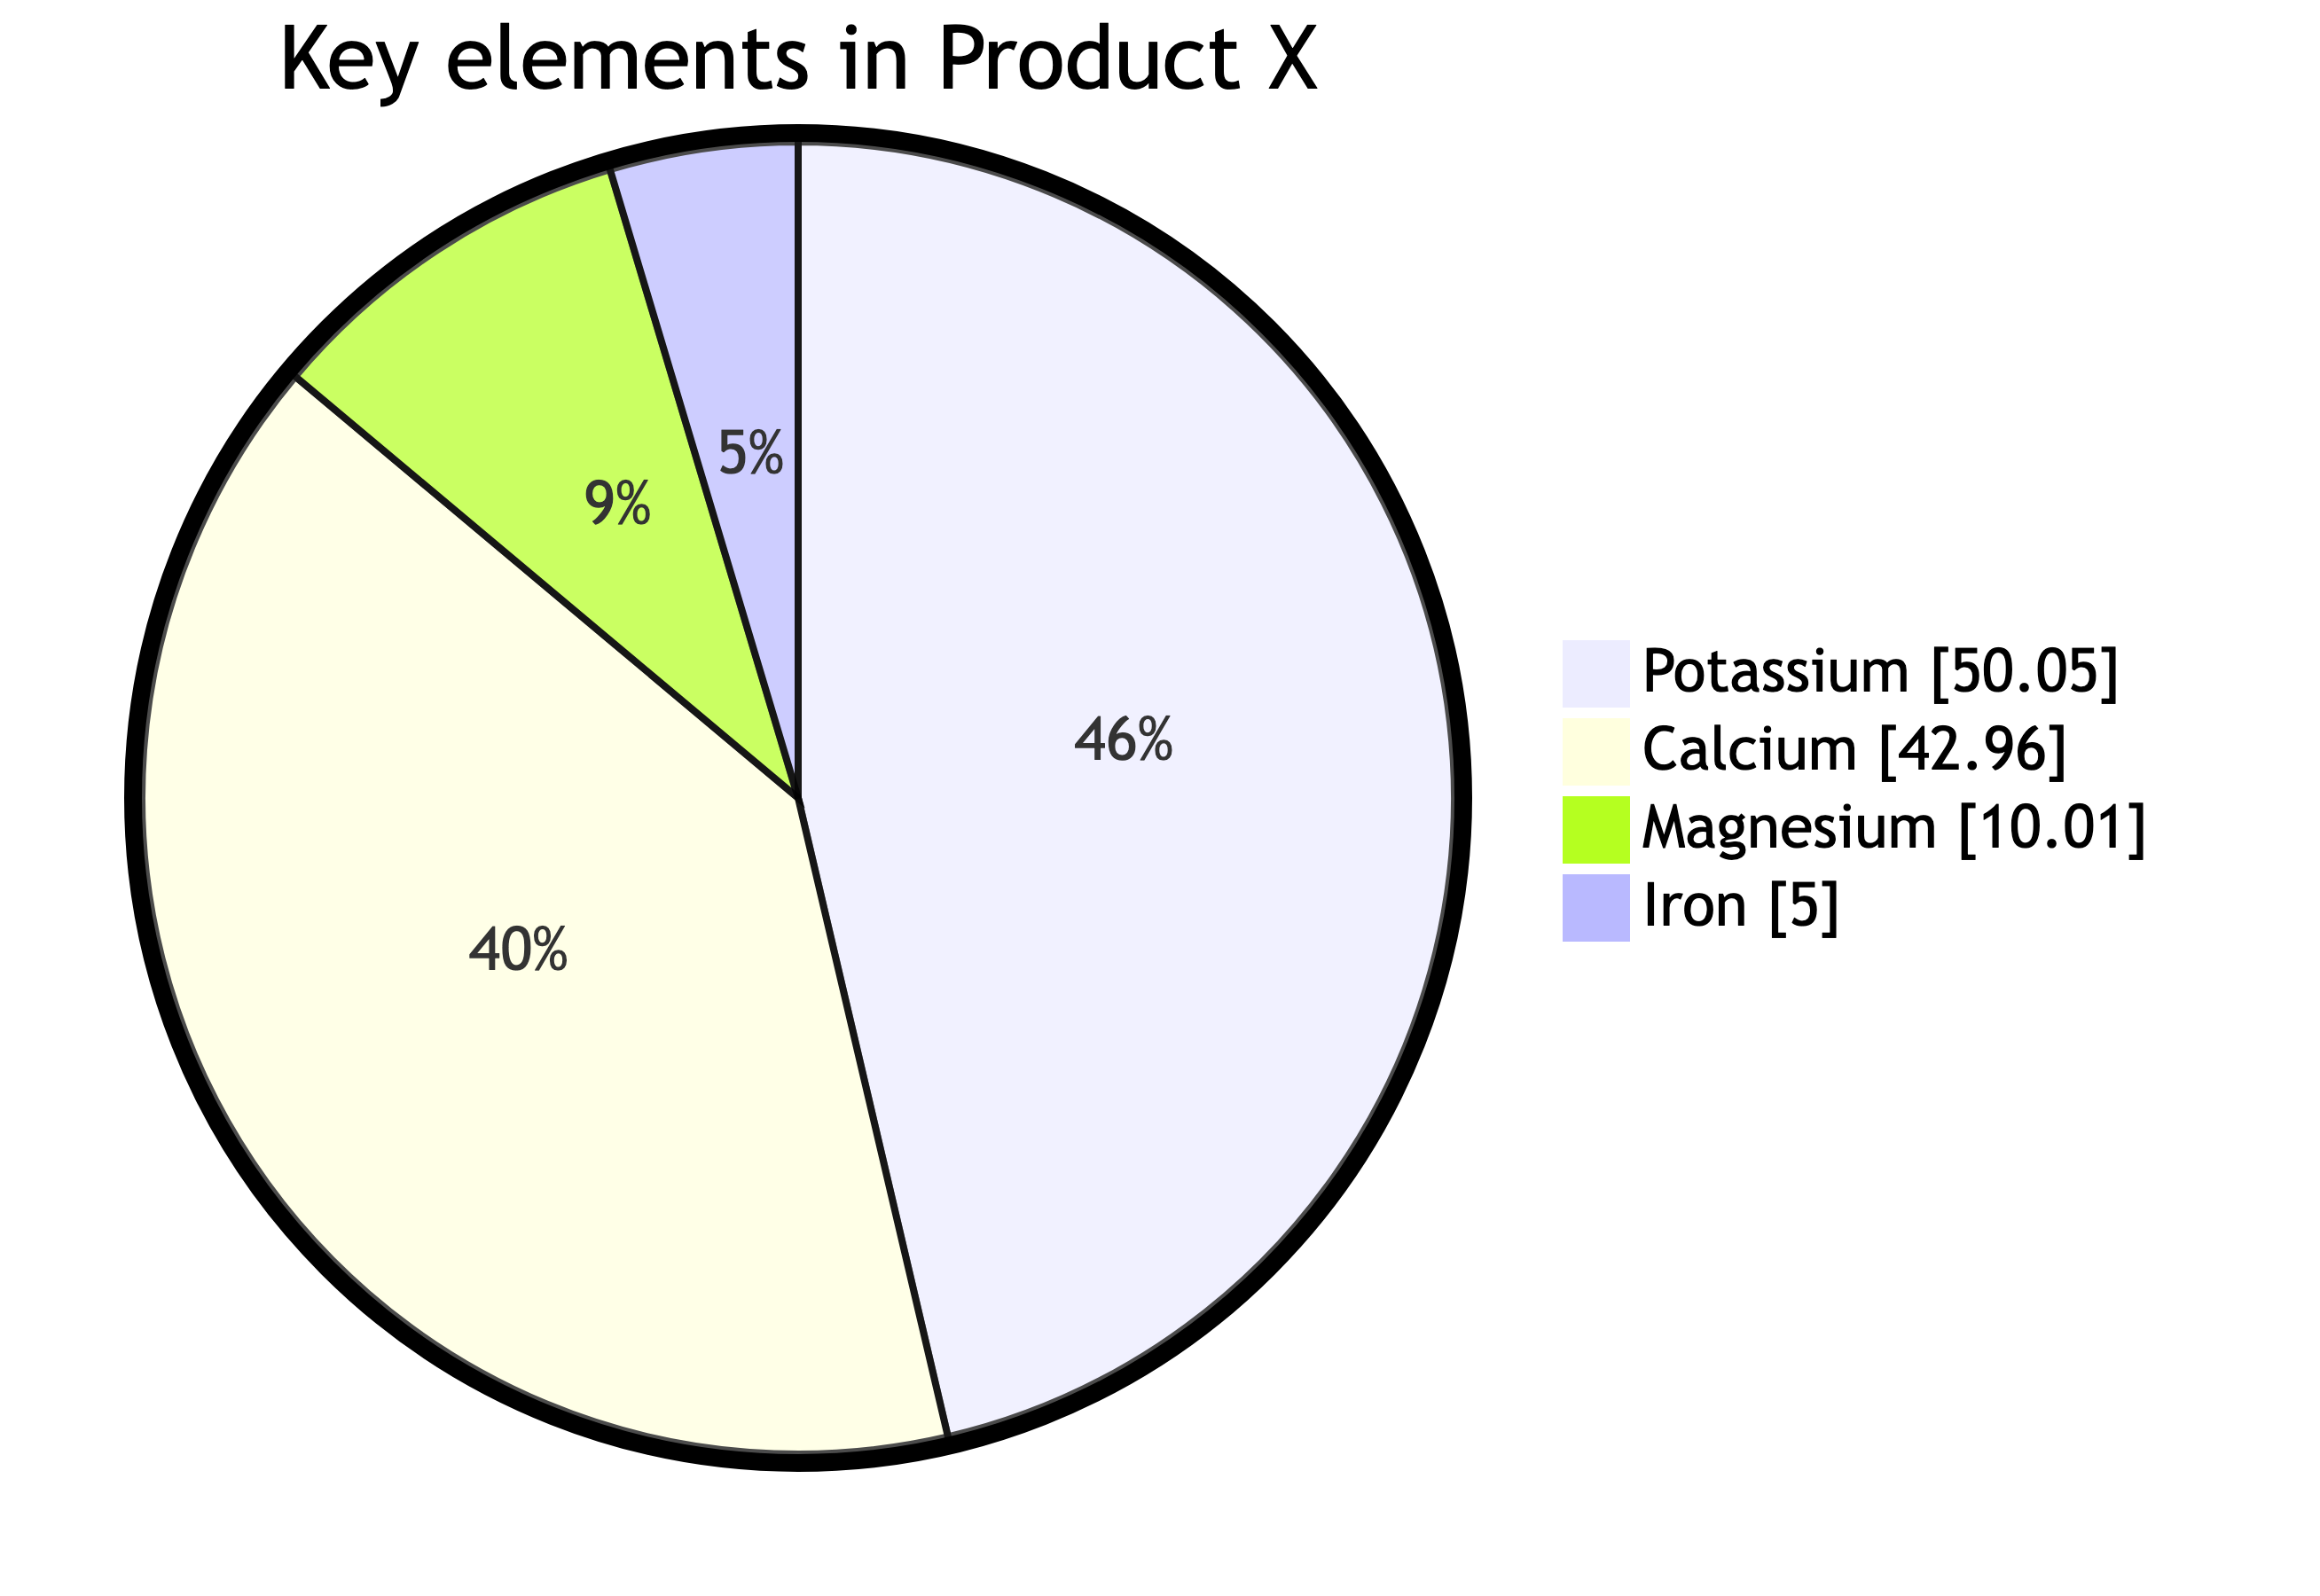
\includegraphics[width=6.82in,height=4.69in]{ScrivQ24_files/figure-latex/mermaid-figure-2.png}

}

\caption{\label{fig-mermaid-c}A Mermaid figure using a Scrivener Section
Type {[}Computation{]} with class {[}mermaid{]}, see
https://quarto.org/docs/authoring/diagrams.html for more details}

\end{figure}%

\section{Equations}\label{equations}

\begin{longtable}[]{@{}ccc@{}}
\toprule\noalign{}
\textbf{Species} & \textbf{Markdown Source} & \textbf{Rendered
Output} \\
\midrule\noalign{}
\endfirsthead
\toprule\noalign{}
\textbf{Species} & \textbf{Markdown Source} & \textbf{Rendered
Output} \\
\midrule\noalign{}
\endhead
\bottomrule\noalign{}
\tabularnewline
\caption{Cross-referencing
\textbf{equations}.}\label{tbl-equations}\tabularnewline
\endlastfoot
Equation & \texttt{{[}@eq-demo-a{]}} &
\phantomsection\label{cite_49}{\label{cite_49}Equation~\ref{eq-demo-a}} \\
Equation & \texttt{{[}@eq-demo-b{]}} &
\phantomsection\label{cite_50}{\label{cite_50}Equation~\ref{eq-demo-b}} \\
\end{longtable}

\begin{equation}\phantomsection\label{eq-demo-a}{t' = \frac{t - \dfrac{v}{c^{2}}x}{\sqrt{1 - \dfrac{v^{2}}{c^{2}}}}}\end{equation}

\begin{equation}\phantomsection\label{eq-demo-b}{t' = \frac{t - \dfrac{v}{c^{2}}x}{\sqrt{1 - \dfrac{v^{2}}{c^{2}}}}
}\end{equation}

\section{Figures}\label{figures}

\begin{longtable}[]{@{}ccc@{}}
\toprule\noalign{}
\textbf{Species} & \textbf{Markdown Source} & \textbf{Rendered
Output} \\
\midrule\noalign{}
\endfirsthead
\toprule\noalign{}
\textbf{Species} & \textbf{Markdown Source} & \textbf{Rendered
Output} \\
\midrule\noalign{}
\endhead
\bottomrule\noalign{}
\tabularnewline
\caption{Cross-referencing figures.}\label{tbl-figures}\tabularnewline
\endlastfoot
& \texttt{{[}@fig-ulysses{]}} &
\phantomsection\label{cite_51}{\label{cite_51}Figure~\ref{fig-ulysses}} \\
Multipart Figure & \texttt{{[}@fig-panel-a{]}} &
\phantomsection\label{cite_52}{\label{cite_52}Figure~\ref{fig-panel-a}} \\
Multipart Figure & \texttt{{[}@fig-panel-a-item-a{]}} &
\phantomsection\label{cite_53}{\label{cite_53}Figure~\ref{fig-panel-a-item-a}} \\
Multipart Figure & \texttt{{[}@fig-panel-a-item-b{]}} &
\phantomsection\label{cite_54}{\label{cite_54}Figure~\ref{fig-panel-a-item-b}} \\
\end{longtable}

\begin{figure}

\centering{

\pandocbounded{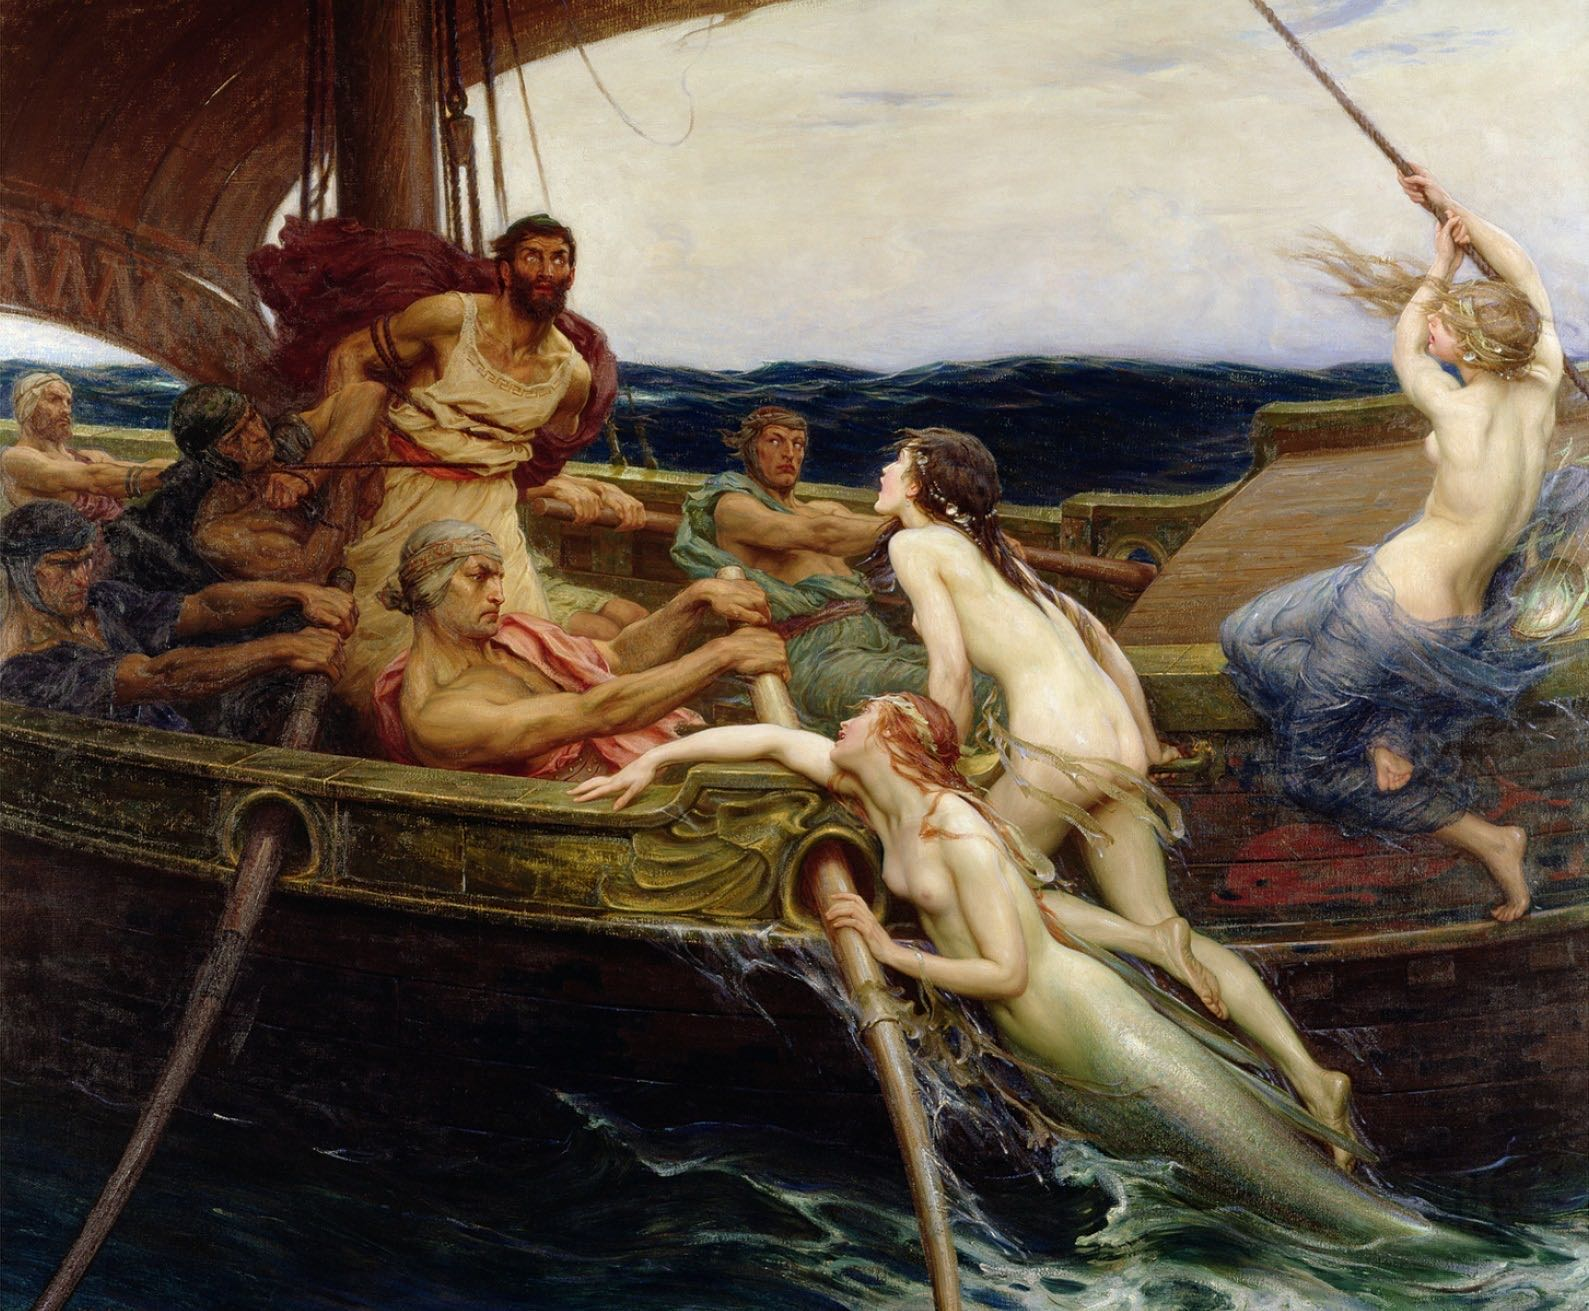
\includegraphics[keepaspectratio]{Ulysses-sirens.jpg}}

}

\caption{\label{fig-ulysses}Ulysses and the Sirens.}

\end{figure}%

Painting by
\phantomsection\label{cite_55}{\label{cite_55}\citeproc{ref-Draper1909}{DRAPER,
1909}}.

\begin{figure*}

\begin{minipage}{0.50\linewidth}

\centering{

\pandocbounded{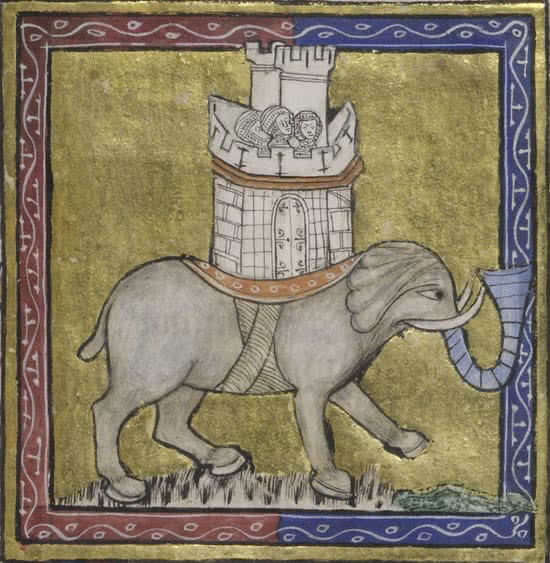
\includegraphics[keepaspectratio]{Elephant2.jpg}}

}

\subcaption{\label{fig-panel-a-item-a}Place the label first in the
caption, and use the \texttt{Caption} style.}

\end{minipage}%
%
\begin{minipage}{0.50\linewidth}

\centering{

\pandocbounded{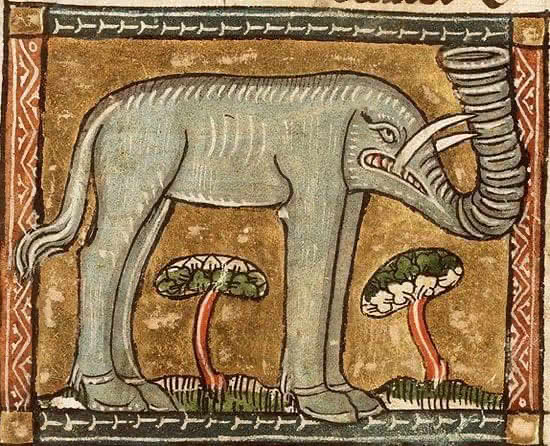
\includegraphics[keepaspectratio]{Elephant3.jpg}}

}

\subcaption{\label{fig-panel-a-item-b}Angry elephant with a big trunk.}

\end{minipage}%

\caption{\label{fig-panel-a}This multi-figure panel uses the
\textbf{Section Type} \texttt{Div} instead of raw markdown as shown
here. \texttt{ID}, \texttt{Class}, and \texttt{Attributes} specific to
the block
{[}\texttt{\#fig-panel-a\ .column-body\ layout-ncol=2\ layout-valign="bottom"}{]}
are saved to
\texttt{Custom\ Metadata-\textgreater{}ID,\ Class\ \&\ Attributes}, and
then inserted into the markup for this chunk by the Section Layout at
compile time.}

\end{figure*}%

\section{Listings}\label{listings}

\begin{longtable}[]{@{}ccc@{}}
\toprule\noalign{}
\textbf{Species} & \textbf{Markdown Source} & \textbf{Rendered
Output} \\
\midrule\noalign{}
\endfirsthead
\toprule\noalign{}
\textbf{Species} & \textbf{Markdown Source} & \textbf{Rendered
Output} \\
\midrule\noalign{}
\endhead
\bottomrule\noalign{}
\tabularnewline
\caption{Cross-referencing listings.}\label{tbl-listings}\tabularnewline
\endlastfoot
Listing & \texttt{{[}@lst-demo-a{]}} &
\phantomsection\label{cite_56}{\label{cite_56}Listing~\ref{lst-demo-a}} \\
Listing & \texttt{{[}@lst-demo-b{]}} &
\phantomsection\label{cite_57}{\label{cite_57}Listing~\ref{lst-demo-b}} \\
\end{longtable}

\begin{codelisting}

\caption{\label{lst-demo-a}Decomposition of Unicode characters.}

\centering{

\begin{Shaded}
\begin{Highlighting}[]
\FunctionTok{require} \StringTok{"unicode/name"}

\NormalTok{characters }\KeywordTok{=}\OtherTok{ \%w(}\StringTok{α β ἇ ᾇ ᾁ}\OtherTok{)}

\CommentTok{\# characters = \textquotesingle{}ἄ\textquotesingle{}}
\NormalTok{characters}\AttributeTok{.each} \ControlFlowTok{do} \KeywordTok{|}\NormalTok{character}\KeywordTok{|}
  \FunctionTok{puts}\NormalTok{ character}\AttributeTok{.unpack}\NormalTok{(}\VerbatimStringTok{\textquotesingle{}U*\textquotesingle{}}\NormalTok{)}\AttributeTok{.map} \KeywordTok{\{} \KeywordTok{|}\NormalTok{i}\KeywordTok{|} 
  \StringTok{"U+}\SpecialCharTok{\#\{}\NormalTok{i}\AttributeTok{.to\_s}\NormalTok{(}\DecValTok{16}\NormalTok{)}\AttributeTok{.rjust}\NormalTok{(}\DecValTok{4}\NormalTok{, }\CharTok{\textquotesingle{}0\textquotesingle{}}\NormalTok{)}\AttributeTok{.upcase}\SpecialCharTok{\}}\StringTok{"}
  \KeywordTok{\}}\AttributeTok{.join}
  \FunctionTok{puts} \DataTypeTok{Unicode}\KeywordTok{::}\DataTypeTok{Name}\AttributeTok{.of}\NormalTok{ character}
\ControlFlowTok{end}
\end{Highlighting}
\end{Shaded}

}

\end{codelisting}%

\begin{codelisting}

\caption{\label{lst-demo-b}The caption}

\centering{

\begin{Shaded}
\begin{Highlighting}[numbers=left,,]
\ControlFlowTok{\#!/usr/bin/env ruby}
\CommentTok{\# frozen\_string\_literal: false}

\DataTypeTok{Encoding}\AttributeTok{.default\_external} \KeywordTok{=} \DataTypeTok{Encoding}\KeywordTok{::}\DataTypeTok{UTF\_8}

\DataTypeTok{Dir}\KeywordTok{[}\StringTok{"}\SpecialCharTok{\#\{}\NormalTok{\_\_dir\_\_}\SpecialCharTok{\}}\StringTok{/Ruby/**/*.rb"}\KeywordTok{]}\AttributeTok{.each} \ControlFlowTok{do} \KeywordTok{|}\NormalTok{file}\KeywordTok{|}
  \FunctionTok{require\_relative}\NormalTok{ file}
\ControlFlowTok{end}
\end{Highlighting}
\end{Shaded}

}

\end{codelisting}%

\section{Tables}\label{tables}

\begin{longtable}[]{@{}ccc@{}}
\toprule\noalign{}
\textbf{Species} & \textbf{Markdown Source} & \textbf{Rendered
Output} \\
\midrule\noalign{}
\endfirsthead
\toprule\noalign{}
\textbf{Species} & \textbf{Markdown Source} & \textbf{Rendered
Output} \\
\midrule\noalign{}
\endhead
\bottomrule\noalign{}
\tabularnewline
\caption{Cross-referencing tables.}\label{tbl-tables}\tabularnewline
\endlastfoot
& \texttt{{[}@tbl-demo-a{]}} &
\phantomsection\label{cite_58}{\label{cite_58}Table~\ref{tbl-demo-a}} \\
& \texttt{{[}@tbl-demo-b{]}} &
\phantomsection\label{cite_59}{\label{cite_59}Table~\ref{tbl-demo-b}} \\
Multipart Table & \texttt{{[}@tbl-panel-a{]}} &
\phantomsection\label{cite_60}{\label{cite_60}Table~\ref{tbl-panel-a}} \\
Multipart Table & \texttt{{[}@tbl-panel-a-item-a{]}} &
\phantomsection\label{cite_61}{\label{cite_61}Table~\ref{tbl-panel-a-item-a}} \\
Multipart Table & \texttt{{[}@tbl-panel-a-item-b{]}} &
\phantomsection\label{cite_62}{\label{cite_62}Table~\ref{tbl-panel-a-item-b}} \\
\end{longtable}

\begin{longtable}[]{@{}cc@{}}
\toprule\noalign{}
\textbf{GRC} & \textbf{SKT} \\
\midrule\noalign{}
\endfirsthead
\toprule\noalign{}
\textbf{GRC} & \textbf{SKT} \\
\midrule\noalign{}
\endhead
\bottomrule\noalign{}
\tabularnewline
\caption{This table with with a passage from John 1.1 uses the
\textbf{Section Type} \ul{Text} and \textbf{Paragraph Style} \ul{Table
Caption}.}\label{tbl-demo-a}\tabularnewline
\endlastfoot
\foreignlanguage{ancientgreek}{ἐν ἀρχὴ ἦν ὁ~λόγος} &
\skt{आदौ वाद आसीत्} \\
\end{longtable}

\begin{longtable}[]{@{}cc@{}}
\toprule\noalign{}
\textbf{GRC} & \textbf{SKT} \\
\midrule\noalign{}
\endfirsthead
\toprule\noalign{}
\textbf{GRC} & \textbf{SKT} \\
\midrule\noalign{}
\endhead
\bottomrule\noalign{}
\tabularnewline
\caption{\enquote{This is an example of \textbf{Section Type}
\texttt{Table}. The caption and the remaining attributes are added as
part of the Section Type markup.}}\label{tbl-demo-b}\tabularnewline
\endlastfoot
\foreignlanguage{ancientgreek}{ἐν ἀρχὴ ἦν ὁ~λόγος} &
\skt{आदौ वाद आसीत्} \\
\end{longtable}

\begin{table}

\begin{minipage}{\linewidth}

\centering{

\begin{tabular}{cccc}
\toprule
\textbf{Element} & \textbf{Prefix} & \textbf{Markdown
Source} & \textbf{Rendered Output}\\
\midrule
Equation A & eq & A & B\\
Equation A & eq & C & D\\
Listing A & lst & E & F\\
\bottomrule
\end{tabular}

}

\subcaption{\label{tbl-panel-a-item-a}The first table of the multipart
table panel.}

\end{minipage}%
\newline
\begin{minipage}{\linewidth}

\centering{

\begin{tabular}{cccc}
\toprule
\textbf{Element} & \textbf{Prefix} & \textbf{Markdown
Source} & \textbf{Rendered Output}\\
\midrule
Equation B & eq & A & B\\
Equation B & eq & C & D\\
Listing B & lst & E & F\\
\bottomrule
\end{tabular}

}

\subcaption{\label{tbl-panel-a-item-b}The second table of the multipart
table panel.}

\end{minipage}%

\caption{\label{tbl-panel-a}This is a markdown multi-table panel with
two sub-tables generated using a \textbf{Section Type} \texttt{Div}. The
\textbf{Custom Metadata} holds the cross-referencing label, classes, and
other attributes.}

\end{table}%

\section{Sections}\label{sec-dem}

\begin{longtable}[]{@{}ccc@{}}
\toprule\noalign{}
\textbf{Genus} & \textbf{Markdown Source} & \textbf{Rendered Output} \\
\midrule\noalign{}
\endfirsthead
\toprule\noalign{}
\textbf{Genus} & \textbf{Markdown Source} & \textbf{Rendered Output} \\
\midrule\noalign{}
\endhead
\bottomrule\noalign{}
\tabularnewline
\caption{Note that the unnumbered section cannot be
referenced.}\label{tbl-sections}\tabularnewline
\endlastfoot
Section & \texttt{{[}@sec-demo-a{]}} &
\phantomsection\label{cite_63}{\label{cite_63}Section~\ref{sec-demo-a}} \\
Break + Section & \texttt{{[}@sec-demo-e{]}} &
\phantomsection\label{cite_64}{\label{cite_64}Section~\ref{sec-demo-e}} \\
Heading & \texttt{{[}@sec-demo-c{]}} &
\phantomsection\label{cite_65}{\label{cite_65}Section~\ref{sec-demo-c}} \\
Break + Heading & \texttt{{[}@sec-demo-d{]}} &
\phantomsection\label{cite_66}{\label{cite_66}Section~\ref{sec-demo-d}} \\
\end{longtable}

\subsection*{Section (Unnumbered)}\label{sec-demo-b}
\addcontentsline{toc}{subsection}{Section (Unnumbered)}

Demonstration of the \textbf{Section Type} \emph{Section} using
\textbf{Class} \texttt{.unnumbered}.

\subsection{Section}\label{sec-demo-a}

Demonstration of the \textbf{Section Type} \emph{Section} with
\textbf{ID} \texttt{\#sec-demo-a}.

\newpage{}

\subsection{Break + Section}\label{sec-demo-e}

Demonstration of the \textbf{Section Type} \emph{Break + Section} with
\textbf{ID} \texttt{\#sec-demo-e}.

\subsection{Heading}\label{sec-demo-c}

\begin{center}\rule{0.5\linewidth}{0.5pt}\end{center}

\subsection{Break + Heading}\label{sec-demo-d}

\chapter{Templates and partials}\label{templates-and-partials}

\begin{tcolorbox}[enhanced jigsaw, bottomrule=.15mm, bottomtitle=1mm, rightrule=.15mm, opacityback=0, coltitle=black, colback=white, left=2mm, arc=.35mm, colbacktitle=quarto-callout-caution-color!10!white, breakable, toptitle=1mm, colframe=quarto-callout-caution-color-frame, toprule=.15mm, titlerule=0mm, title=\textcolor{quarto-callout-caution-color}{\faFire}\hspace{0.5em}{\textbf{Quarto} Templates optionally edited in \textbf{Scrivener}}, leftrule=.75mm, opacitybacktitle=0.6]

Users needing control over the parameters in the native \textbf{Quarto}
templates shouldn't have to deal with external files. We imported all
the templates and partials for the main file types (TeX, HTML, Typst) so
they can be edited directly in Scrivener.

\end{tcolorbox}

\begin{tcolorbox}[enhanced jigsaw, bottomrule=.15mm, bottomtitle=1mm, rightrule=.15mm, opacityback=0, coltitle=black, colback=white, left=2mm, arc=.35mm, colbacktitle=quarto-callout-note-color!10!white, breakable, toptitle=1mm, colframe=quarto-callout-note-color-frame, toprule=.15mm, titlerule=0mm, title=\textcolor{quarto-callout-note-color}{\faInfo}\hspace{0.5em}{PDF}, leftrule=.75mm, opacitybacktitle=0.6]

\begin{itemize}
\tightlist
\item
  \href{_extensions/templates/tex/doc-class.tex}{doc-class}
\item
  \href{_extensions/templates/tex/title.tex}{title}
\item
  \href{_extensions/templates/tex/toc.tex}{toc}
\item
  \href{_extensions/templates/tex/before-body.tex}{before-body}
\item
  \href{_extensions/templates/tex/before-bib.tex}{before-bib}
\item
  \href{_extensions/templates/tex/biblio.tex}{biblio}
\item
  \href{_extensions/templates/tex/after-body.tex}{after-body}
\end{itemize}

And the Pandoc sub-partials:

\begin{itemize}
\tightlist
\item
  \href{_extensions/templates/tex/tightlist.tex}{tightlist}
\item
  \href{_extensions/templates/tex/tables.tex}{tables}
\item
  \href{_extensions/templates/tex/graphics.tex}{graphics}
\item
  \href{_extensions/templates/tex/citations.tex}{citations}
\end{itemize}

\end{tcolorbox}

\begin{tcolorbox}[enhanced jigsaw, bottomrule=.15mm, bottomtitle=1mm, rightrule=.15mm, opacityback=0, coltitle=black, colback=white, left=2mm, arc=.35mm, colbacktitle=quarto-callout-note-color!10!white, breakable, toptitle=1mm, colframe=quarto-callout-note-color-frame, toprule=.15mm, titlerule=0mm, title=\textcolor{quarto-callout-note-color}{\faInfo}\hspace{0.5em}{HTML}, leftrule=.75mm, opacitybacktitle=0.6]

\begin{itemize}
\tightlist
\item
  \href{_extensions/templates/html/title-block.html}{title-block}
\item
  \href{_extensions/templates/html/styles.html}{styles}
\item
  \href{_extensions/templates/html/html.template}{html-template}
\item
  \href{_extensions/templates/html/html.styles}{html-styles}
\item
  \href{_extensions/templates/html/toc.html}{toc}
\item
  \href{_extensions/templates/html/metadata.html}{metadata}
\end{itemize}

\end{tcolorbox}

\chapter{Resources}\label{resources}

\begin{itemize}
\tightlist
\item
  \href{https://icons.getbootstrap.com}{Bootstrap Icons} - These are
  available in Quarto documents using the \textbf{Shortcode Font
  Awesome} style as in \texttt{} \faIcon{bell}. (There is also
  \textbf{Shortcode Env}, \textbf{Shortcode Meta}, \textbf{Shortcode
  Var}).
\item
  \href{https://plain-text.co/index.html\#introduction}{The Plain
  Person's Guide to Plain Text Social Science}
\item
  \href{https://quarto.org/docs/reference/}{Quarto Reference}
\item
  The easiest way to
  \href{quarto.org/docs/publishing/github-pages.html\#render-to-docs}{publish
  to Github Pages}
\item
  \href{https://github.com/jjallaire/hopr/blob/master/_quarto.yml}{Example
  of Quarto Book}
\item
  \href{https://tarleb.com/posts/quarto-with-gh-pages/}{Quarto with GH
  Pages}
\end{itemize}

\chapter{Final word}\label{final-word}

If you like what you see, consider sponsoring
\href{https://github.com/sponsors/bcdavasconcelos}{this project on
Github}.

\begin{tcolorbox}[enhanced jigsaw, bottomrule=.15mm, bottomtitle=1mm, rightrule=.15mm, opacityback=0, coltitle=black, colback=white, left=2mm, arc=.35mm, colbacktitle=quarto-callout-warning-color!10!white, breakable, toptitle=1mm, colframe=quarto-callout-warning-color-frame, toprule=.15mm, titlerule=0mm, title=\textcolor{quarto-callout-warning-color}{\faExclamationTriangle}\hspace{0.5em}{Known problems \& random errors}, leftrule=.75mm, opacitybacktitle=0.6]

\begin{itemize}
\tightlist
\item
  Compilation fails for \textbf{LaTeX → PDF} when citations are placed
  in Table/Figure captions. The cause seems to be the \textbf{Citation
  Backlinks} filter.
\item
  For \textbf{Typst → PDF} output some \textbf{Quarto} features
  (\emph{e.g.} margin notes, column classes) are not yet implemented.
  Hopefully this will change in future Quarto versions.
\end{itemize}

\end{tcolorbox}

\chapter*{Bibliography}\label{bibliography}
\addcontentsline{toc}{chapter}{Bibliography}

\section*{Primary Sources}\label{sec-primary-sources}
\addcontentsline{toc}{section}{Primary Sources}

\phantomsection\label{refs_primary-sources}
\begin{CSLReferences}{0}{1}
\bibitem[\citeproctext]{ref-DA}
ARISTOTELIS. {``De Anima''}. Em: BEKKER, I. (Ed.). \emph{Aristotelis
Opera}. Trad.: Β. Τατάκης. Berlin: Reimer, 1834.
{[}\Acrobatmenu{GoBack}{$\hookleftarrow$},
\hyperref[cite_13]{\pageref{cite_13}},
\hyperref[cite_14]{\pageref{cite_14}},
\hyperref[cite_15]{\pageref{cite_15}},
\hyperref[cite_16]{\pageref{cite_16}},
\hyperref[cite_17]{\pageref{cite_17}},
\hyperref[cite_18]{\pageref{cite_18}},
\hyperref[cite_19]{\pageref{cite_19}},
\hyperref[cite_20]{\pageref{cite_20}},
\hyperref[cite_21]{\pageref{cite_21}},
\hyperref[cite_22]{\pageref{cite_22}},
\hyperref[cite_23]{\pageref{cite_23}},
\hyperref[cite_24]{\pageref{cite_24}},
\hyperref[cite_25]{\pageref{cite_25}}{]}

\end{CSLReferences}

\section*{Secondary Sources}\label{sec-secondary-sources}
\addcontentsline{toc}{section}{Secondary Sources}

\phantomsection\label{refs_secondary-sources}
\begin{CSLReferences}{0}{1}
\bibitem[\citeproctext]{ref-DABiehl}
ARISTOTELIS. \emph{De Anima}. Ed: W. Biehl. Leipzig: Teubner, 1896.
{[}\Acrobatmenu{GoBack}{$\hookleftarrow$},
\hyperref[cite_26]{\pageref{cite_26}},
\hyperref[cite_27]{\pageref{cite_27}}{]}

\bibitem[\citeproctext]{ref-DATheiler}
ARISTOTELIS. \emph{De Anima}. Ed: W. Biehl. Trads.: Willy Theiler \&
Horst Seidl. Harmburg: Felix Meiner, 1995.
{[}\Acrobatmenu{GoBack}{$\hookleftarrow$},
\hyperref[cite_28]{\pageref{cite_28}},
\hyperref[cite_29]{\pageref{cite_29}}{]}

\bibitem[\citeproctext]{ref-Long2004}
LONG, C. \emph{Ethics of Ontology}. Albany: SUNY, 2004.
{[}\Acrobatmenu{GoBack}{$\hookleftarrow$},
\hyperref[cite_5]{\pageref{cite_5}},
\hyperref[cite_6]{\pageref{cite_6}},
\hyperref[cite_7]{\pageref{cite_7}},
\hyperref[cite_8]{\pageref{cite_8}},
\hyperref[cite_9]{\pageref{cite_9}},
\hyperref[cite_10]{\pageref{cite_10}},
\hyperref[cite_11]{\pageref{cite_11}}{]}

\end{CSLReferences}

\section*{Workflow}\label{sec-workflow}
\addcontentsline{toc}{section}{Workflow}

\phantomsection\label{refs_workflow}
\begin{CSLReferences}{0}{1}
\bibitem[\citeproctext]{ref-hoffman2014}
HOFFMAN, D. D.; PRAKASH, C.
\href{https://doi.org/10.3389/fpsyg.2014.00577}{Objects of
consciousness}. \emph{Frontiers in Psychology}, v. 5, p. 577, 2014.
{[}\Acrobatmenu{GoBack}{$\hookleftarrow$},
\hyperref[cite_12]{\pageref{cite_12}}{]}

\end{CSLReferences}

\section*{Songs}\label{sec-songs}
\addcontentsline{toc}{section}{Songs}

\phantomsection\label{refs_songs}
\begin{CSLReferences}{0}{1}
\bibitem[\citeproctext]{ref-MorphineCFP}
MORPHINE et al. \emph{Cure For Pain}. : Cure For Pain.Rykodisc, 1993.
Disponível em:
\textless{}\url{https://open.spotify.com/track/3hO9gaVixKDoYDrlTBrEWf?si=0668baf1aab345d4}\textgreater{}
{[}\Acrobatmenu{GoBack}{$\hookleftarrow$},
\hyperref[cite_2]{\pageref{cite_2}},
\hyperref[cite_3]{\pageref{cite_3}},
\hyperref[cite_4]{\pageref{cite_4}}{]}

\end{CSLReferences}

\section*{Paintings}\label{sec-paintings}
\addcontentsline{toc}{section}{Paintings}

\phantomsection\label{refs_paintings}
\begin{CSLReferences}{0}{1}
\bibitem[\citeproctext]{ref-Draper1909}
DRAPER, H. J. \emph{Ulysses and the Sirens}., 1909.
{[}\Acrobatmenu{GoBack}{$\hookleftarrow$},
\hyperref[cite_55]{\pageref{cite_55}}{]}

\end{CSLReferences}


\backmatter


\end{document}
